\documentclass[a4paper,zihao=5,UTF8]{ctexart}
\usepackage[top=2.3cm,bottom=2cm,left=1.7cm,right=1.7cm]{geometry} 
\usepackage{amsmath, amssymb}
\usepackage{color}
\usepackage{hyperref} 
\usepackage{pythonhighlight}
\usepackage{listings}
\usepackage{mathrsfs} 
\usepackage{booktabs}
\usepackage{amsthm}
\usepackage{longtable} 
\usepackage{graphicx}
\usepackage{subfigure}
\usepackage{caption}
\usepackage{fontspec}
\usepackage{titlesec}
\usepackage{fancyhdr}
\usepackage{latexsym}
\usepackage{subfigure}
\usepackage{braket}
\usepackage{cite}
\usepackage[version=4]{mhchem}
\usepackage{makecell}

\CTEXsetup[format={\Large\bfseries}]{section}
\def\d{\mathrm{d}}
\def\e{\mathrm{e}}
\def\i{\mathrm{i}}
\def\dps{\displaystyle}
\newcommand{\mr}[1]{\mathrm{#1}}
\newcommand{\mb}[1]{\mathbf{#1}}
\newcommand{\dv}[2]{\frac{\d{#1}}{\d{#2}}}
\newcommand{\pdv}[2]{\frac{\partial{#1}}{\partial{#2}}}
\def\degree{$^{\circ}$}
\def\celsius{^{\circ}\mr{C}}
\title{\textbf{机器学习在化学中的应用:上机作业 01}}
\author{王崇斌\;1800011716}
\makeatletter
\makeatother
\begin{document}
	\pagestyle{fancy}
	\pagestyle{fancy}
    \lhead{机器学习在化学中的应用}
	\chead{}
	\rhead{\today}
	\maketitle
    \thispagestyle{fancy}
    \section{背景介绍:岭回归}
    对于给定的一组数据$(\mathbf{X}, \mb{t})$,我们希望用一个有着准确定义的模型$f(\mb{w}, \mb{x})$
    去描述数据的规律和预言将要产生的结果,同时需要一个标准$E(\mb{w}, \mb{x}, \mb{y})$去衡量模型的好坏。(与
    机器学习的定义还差一个提升精确度的手段)那么需要定义清楚两个概念:1.模型如何设计;2.衡量误差的标准如何制定。
    下面我们简要讨论一下线性模型与损失函数。
    \paragraph{线性基函数模型}
    假设我们的模型可以用如下所线性组合形式的函数来描述:
    \begin{equation}
        f(\mb{w}, \mb{x}) = \sum_{k=0}^{M}w_k\phi_k(\mb{x}) = \mb{w}^t\mb{\Phi}(\mb{x})
    \end{equation}
    \paragraph{最小二乘法}
    对于给定数据集$(\mb{X}, \mb{t})$与模型$f(\mb{w},\mb{x})$,可以定义最小二乘的误差函数:
    \begin{equation}
        E_{D}(\mb{w}, \mb{X}, \mb{t}) = \dfrac{1}{2}\sum_{n=1}^{N}(t_n - f(\mb{w}, \mb{x}_n))^2
    \end{equation}
    对于线性模型,上述损失函数可以写为:
    \begin{equation}
        E_{D}(\mb{w}, \mb{X}, \mb{t}) = \dfrac{1}{2}\sum_{n=1}^{N}(t_n - \mb{w}^t\mb{\Phi}(\mb{x}_n))^2
    \end{equation}
    可以从多种角度来理解上述误差函数,最直观的是它描述了数据点距离模型曲线的距离(有点类似与函数空间的$L_2$范数)。
    更重要的是可以从概率论的角度来理解。假设数据是通过实验获得的,实验本身会给数据引入随机误差,假设对于给定的
    $\mb{x}$,测量值$t$作为一个随机变量其概率密度为均值$f(\mb{w}, \mb{x})$,方差为$\beta^{-1}$的正态分布,
    同时,假设对于不同的$\mb{x}$,随机变量$t$是独立的,那么在给定$(\mb{x}_1, ...,\mb{x}_N)$的情况下,
    $(t_1,...,t_n)$的联合分布的密度函数可以表示为:
    \begin{equation}
        p(\mb{t}|\mb{X}, \mb{w}, \mb{\beta}) = \prod_{n=1}^{N}\mathcal{N}(t_n|f(\mb{w}, \mb{x}_n),\beta^{-1})
    \end{equation}
    那么在$\mb{t}$给定的情况下,通过最大化上述概率密度函数,可以给出一种确定参数$\mb{w}$的方法,容易证明
    这将等价于最小二乘函数的最小化。对于线性模型,可以进一步化简,将上述最小化的问题转化为求解线性方程组的问题。
    \paragraph{正则化的最小二乘法}
    有时候我们不希望模型中的参数$\mb{w}$太大,参数太大往往是过拟合的一个特征(同时也会引入更大的数值不稳定性),
    可以将损失函数定义为(其中$\lambda$是一个给定的参数):
    \begin{equation}
        E_r(\mb{w}, \mb{X}, \mb{t}) = \dfrac{1}{2}\sum_{n=1}^{N}(t_n - \mb{w}^t\mb{\Phi}(\mb{x}_n))^2 + \frac{\lambda}{2}\mb{w}^{t}\mb{w}
    \end{equation}
    如果最小化这个损失函数,同样也可以将最小化问题转化为求解线性方程组的问题(这也是线性模型的一个特点),
    进一步得到参数$\lambda$。同样的,这个损失函数也可以通过最大化后验概率(假设$\mb{w}$的先验概率是高斯分布)
    的方法来获取,这里不详细展示具体过程。
    \section{作业部分}
    \paragraph{(1)}:
    以多项式为基函数时,在训练集和测试集上的均方误差随$\lambda$的关系、拟合参数随$\lambda$的关系
    如表 1 所示。
    \begin{table}[htbp]
        \centering
        \label{poly_params}
        \begin{tabular}[htbp]{cc}
            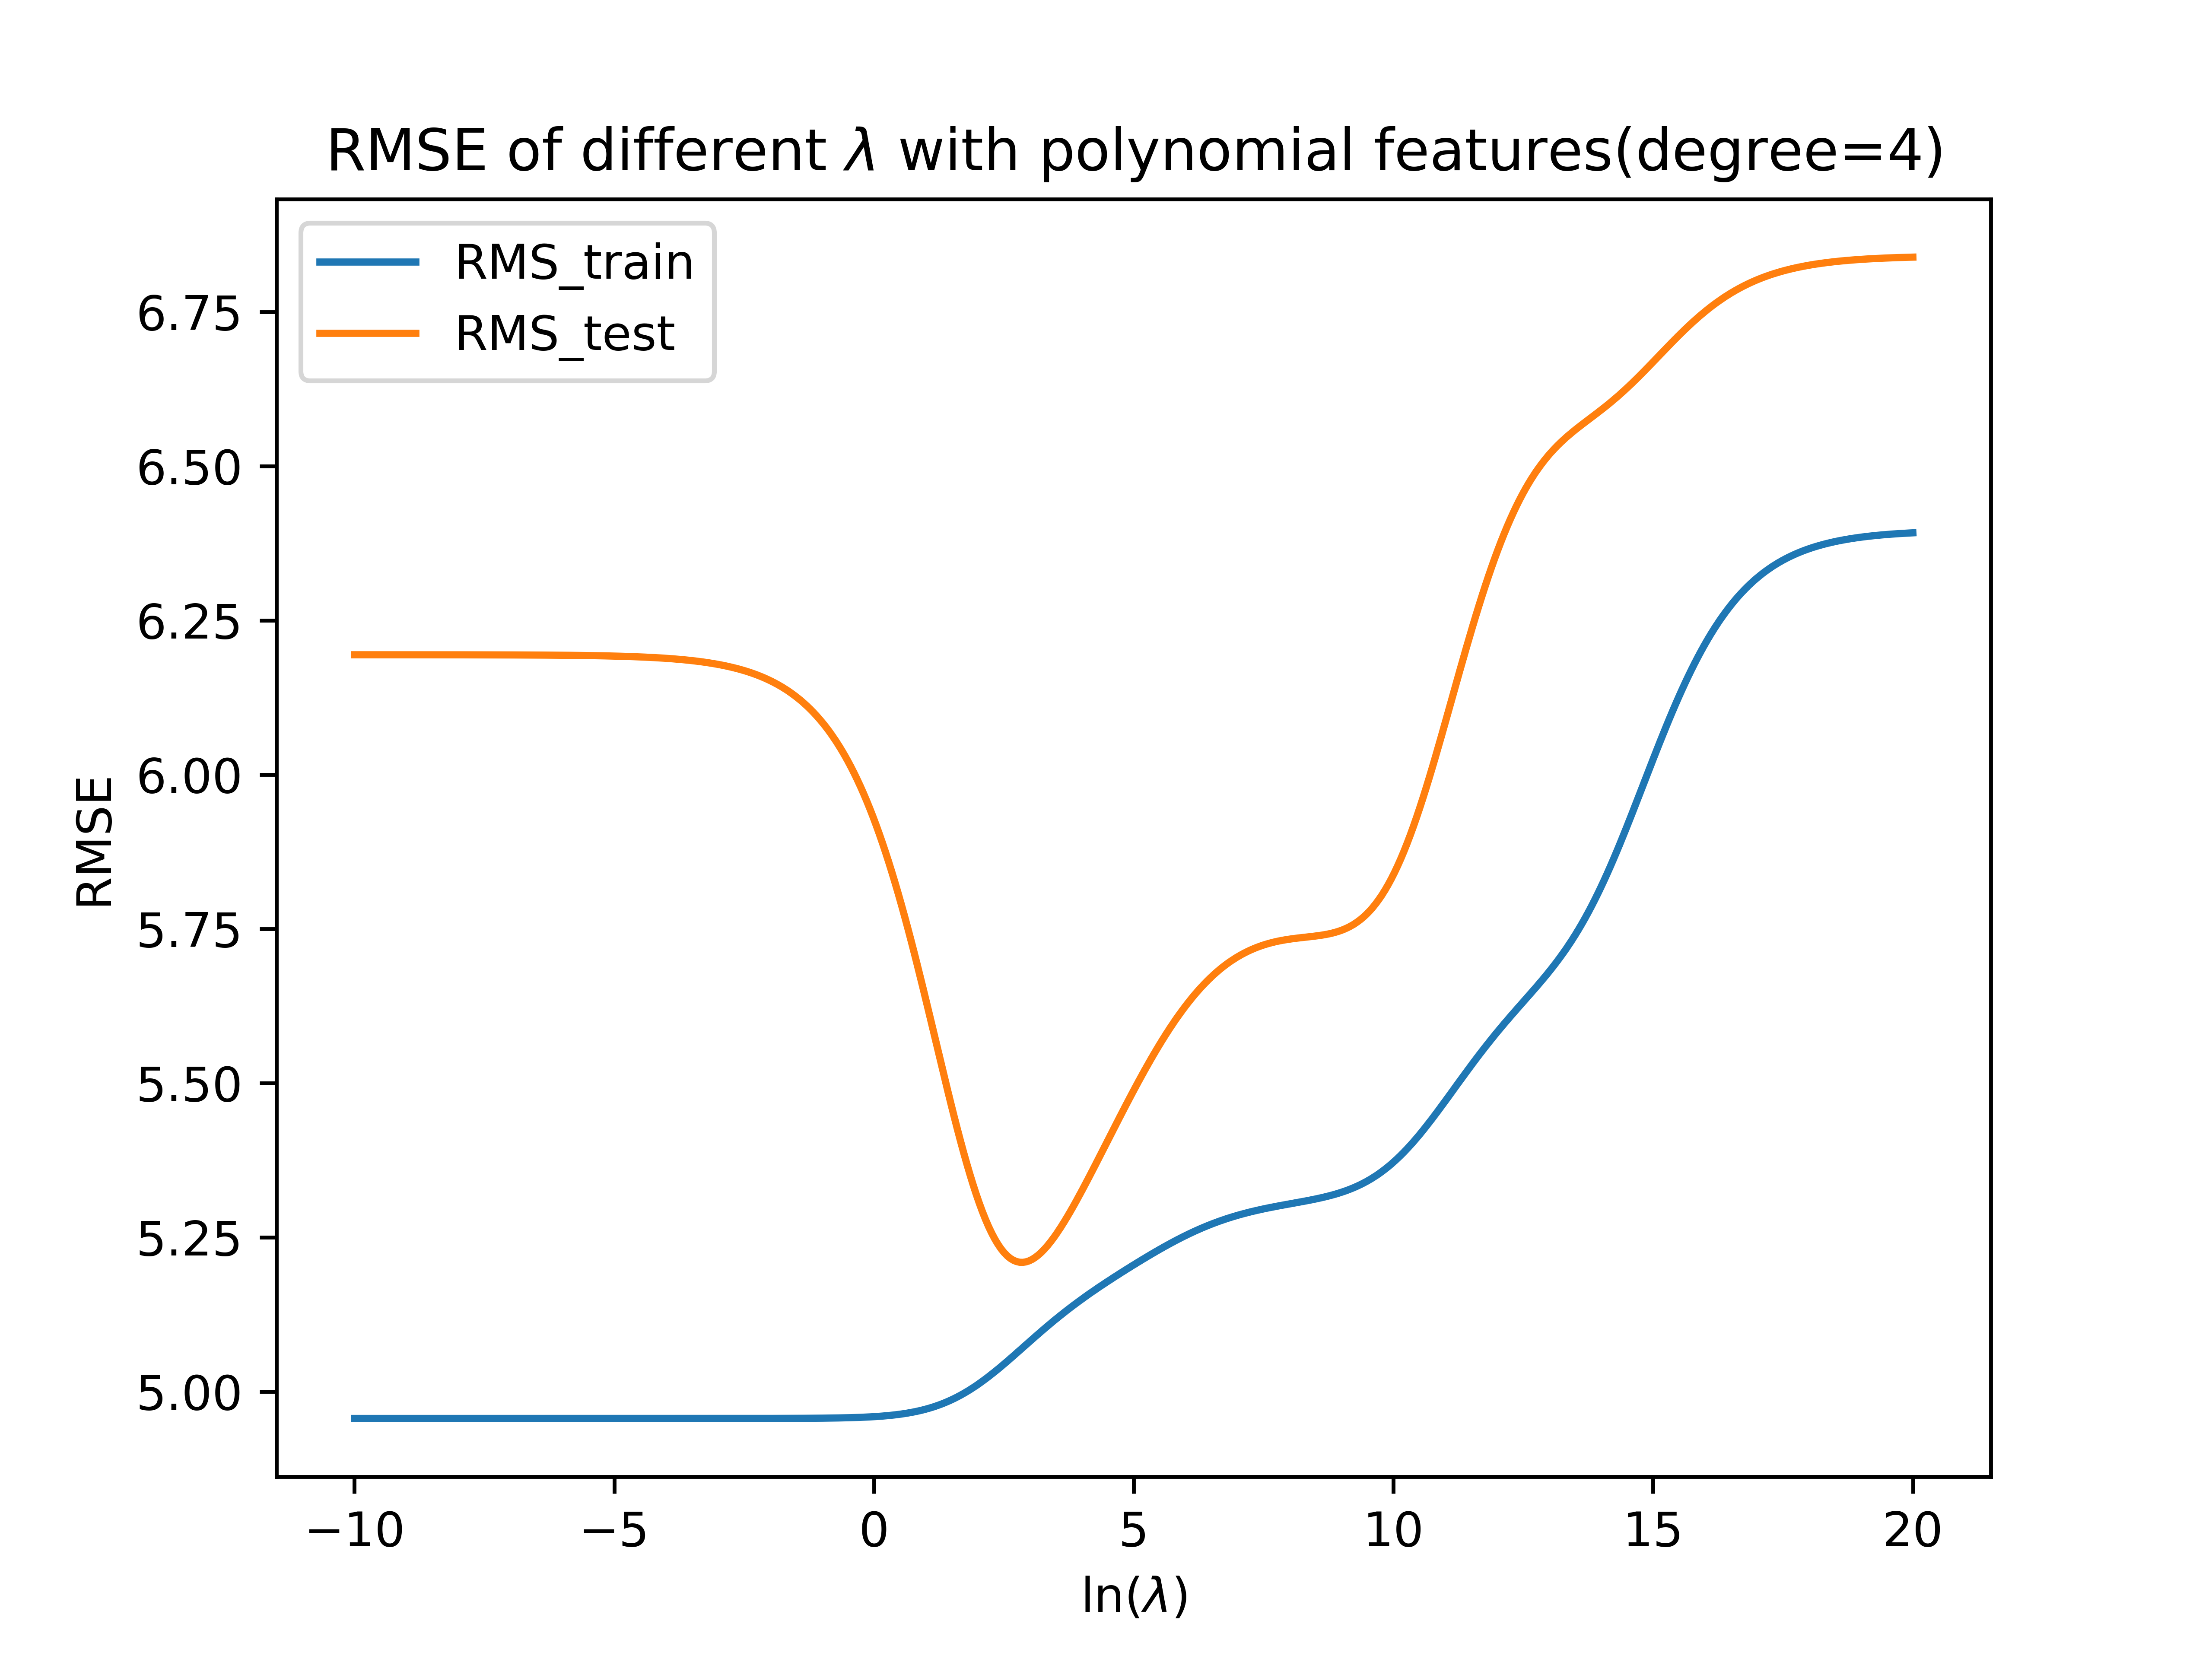
\includegraphics[scale=0.5]{RMSE_polynomials.png} & 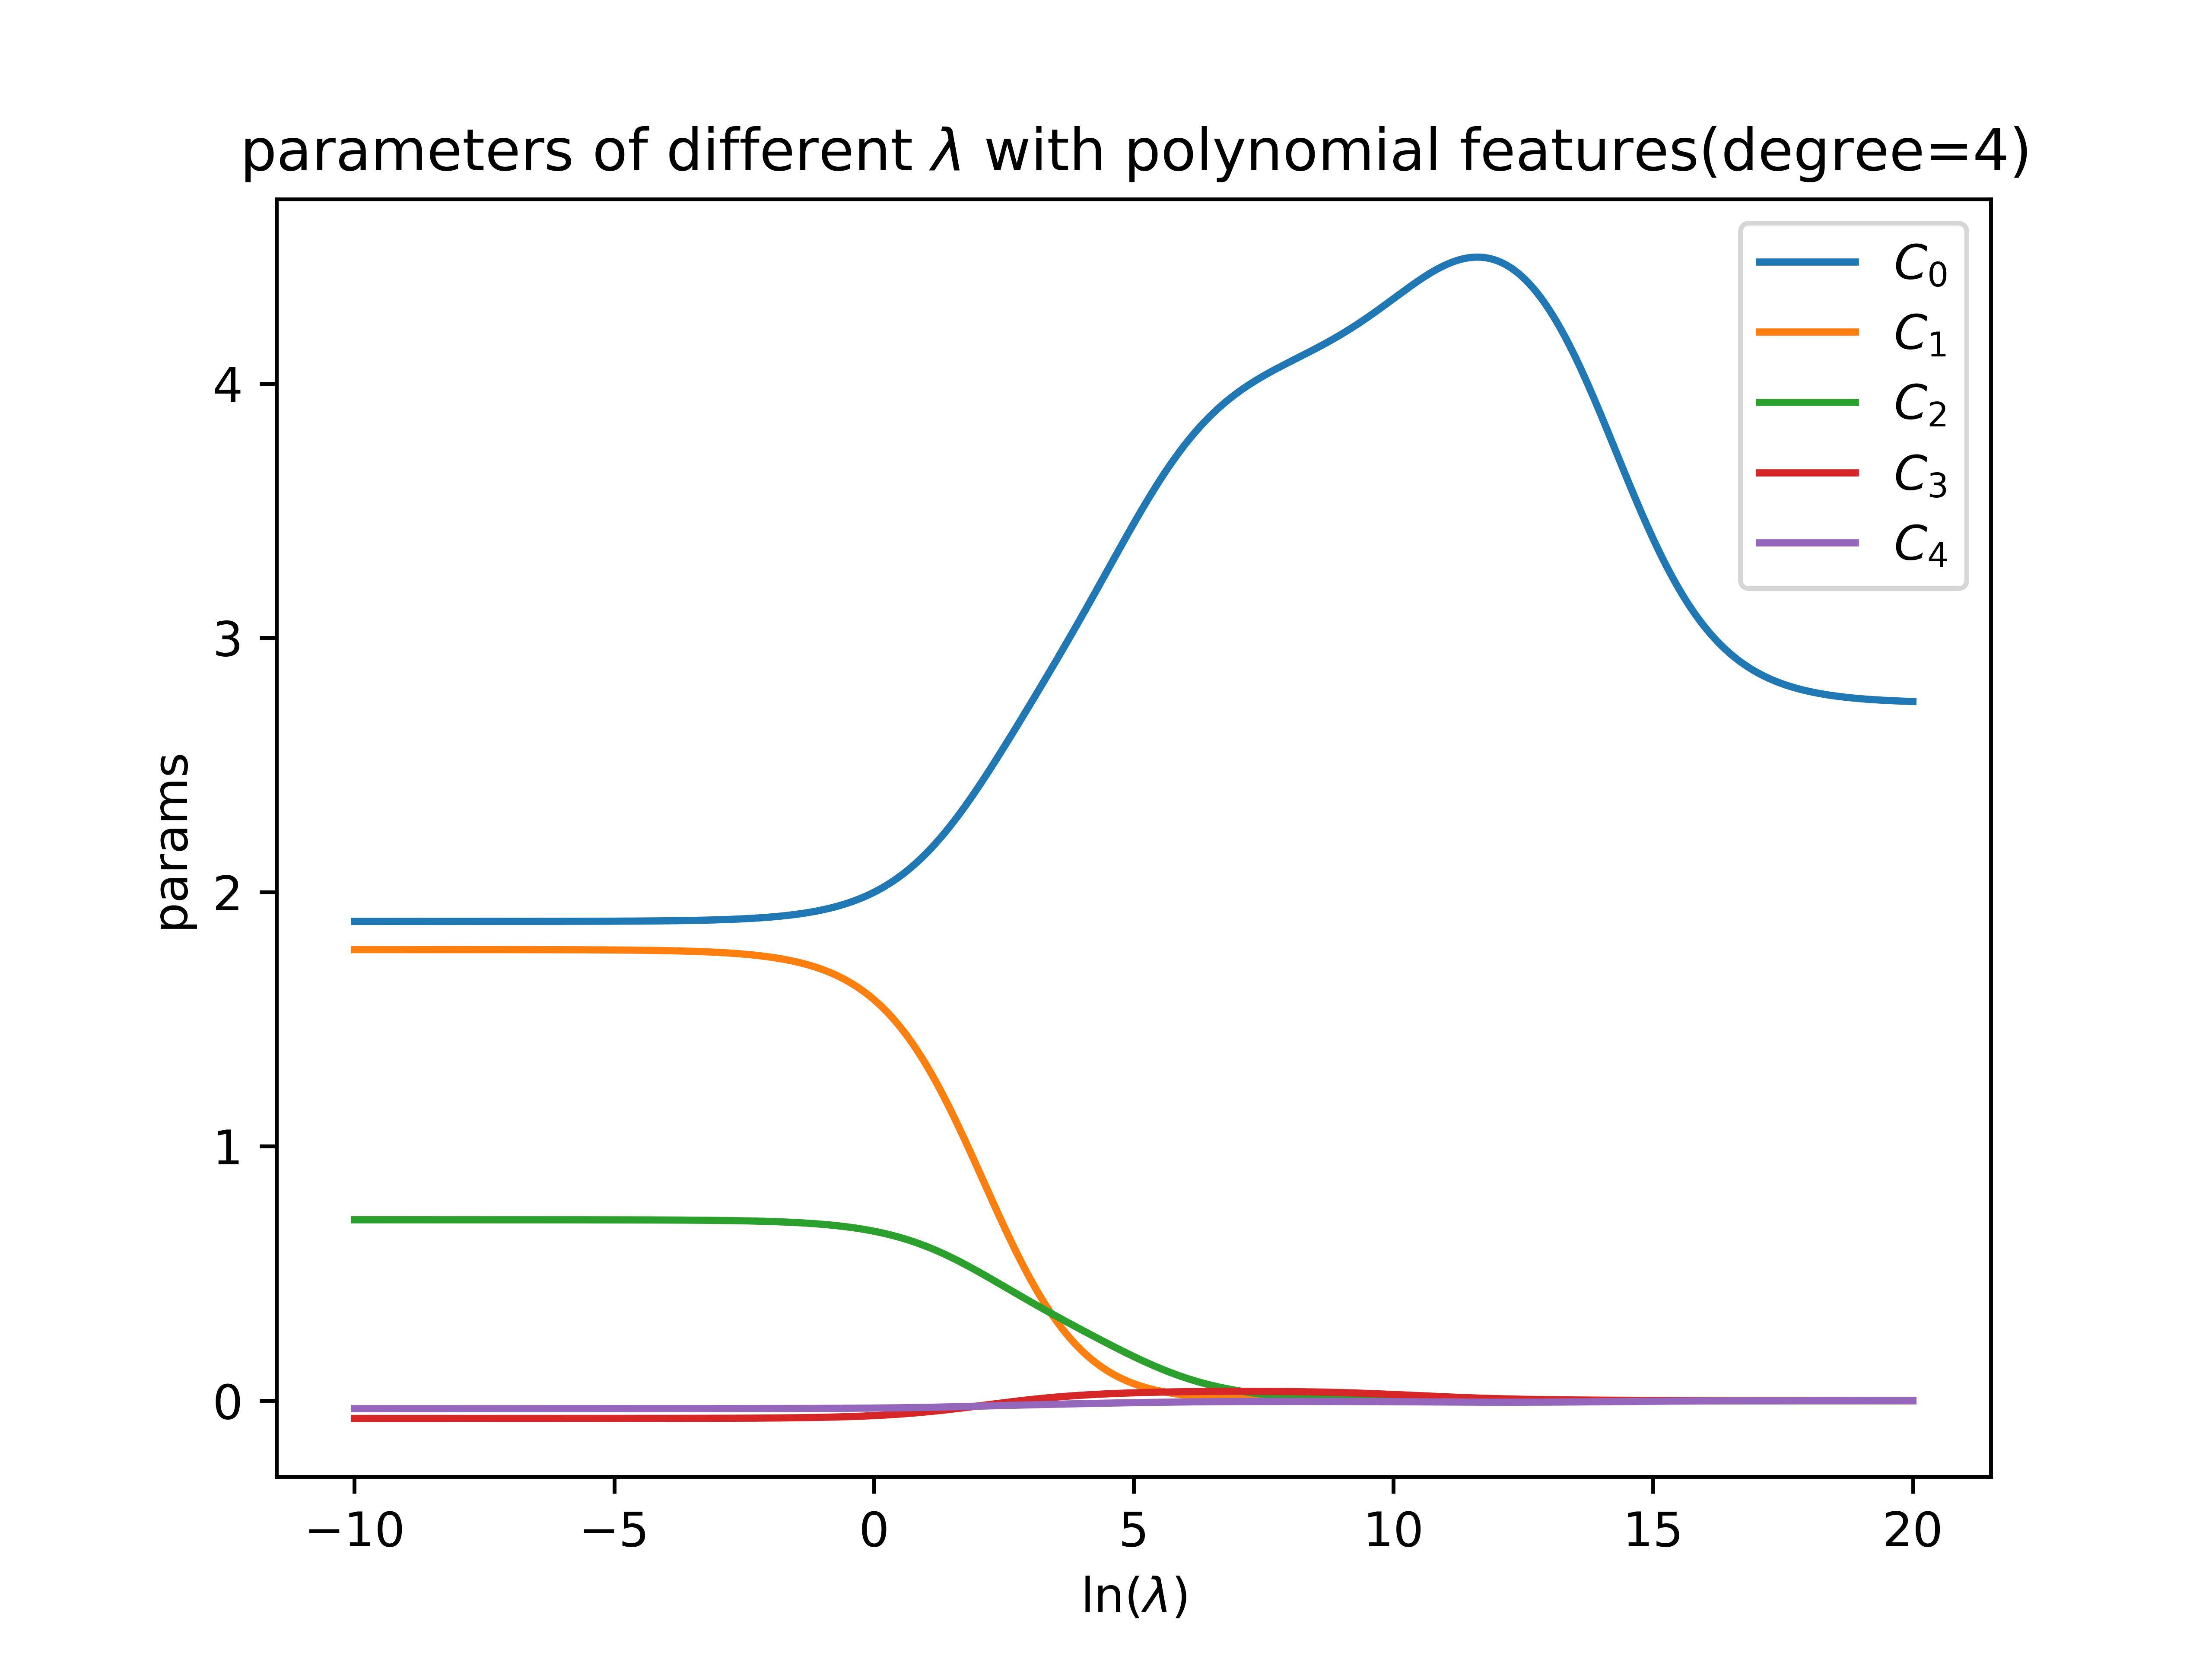
\includegraphics[scale=0.5]{Params_polynomials.png} \\
        \end{tabular}
        \caption{多项式为基函数时均方误差与拟合参数随超参数的关系}
    \end{table}
    \paragraph{(2)}:
    从表 1 可以看出,当$\ln(\lambda) = 2.5$左右时,可以在训练集和测试集上都得到一个比较小的
    均方误差,选定这个参数。得到表 2 的数据
    \begin{table}[htbp]
        \centering
        \caption{最佳超参数下的多项式拟合数据}
        \begin{tabular}[htbp]{ccccccc}
            \toprule
            RMSE-train & RMSE-test & $C_0$ & $C_1$ & $C_2$ & $C_3$ & $C_4$\\
            \midrule
            5.0445 & 5.2261 & 2.5690 & 0.6870 & 0.4498 & -0.0081 & -0.0192 \\
            \bottomrule
        \end{tabular}
        \label{poly curve table}
    \end{table}
    同时给出拟合图像图 1。
    \begin{figure}[htbp]
        \centering
        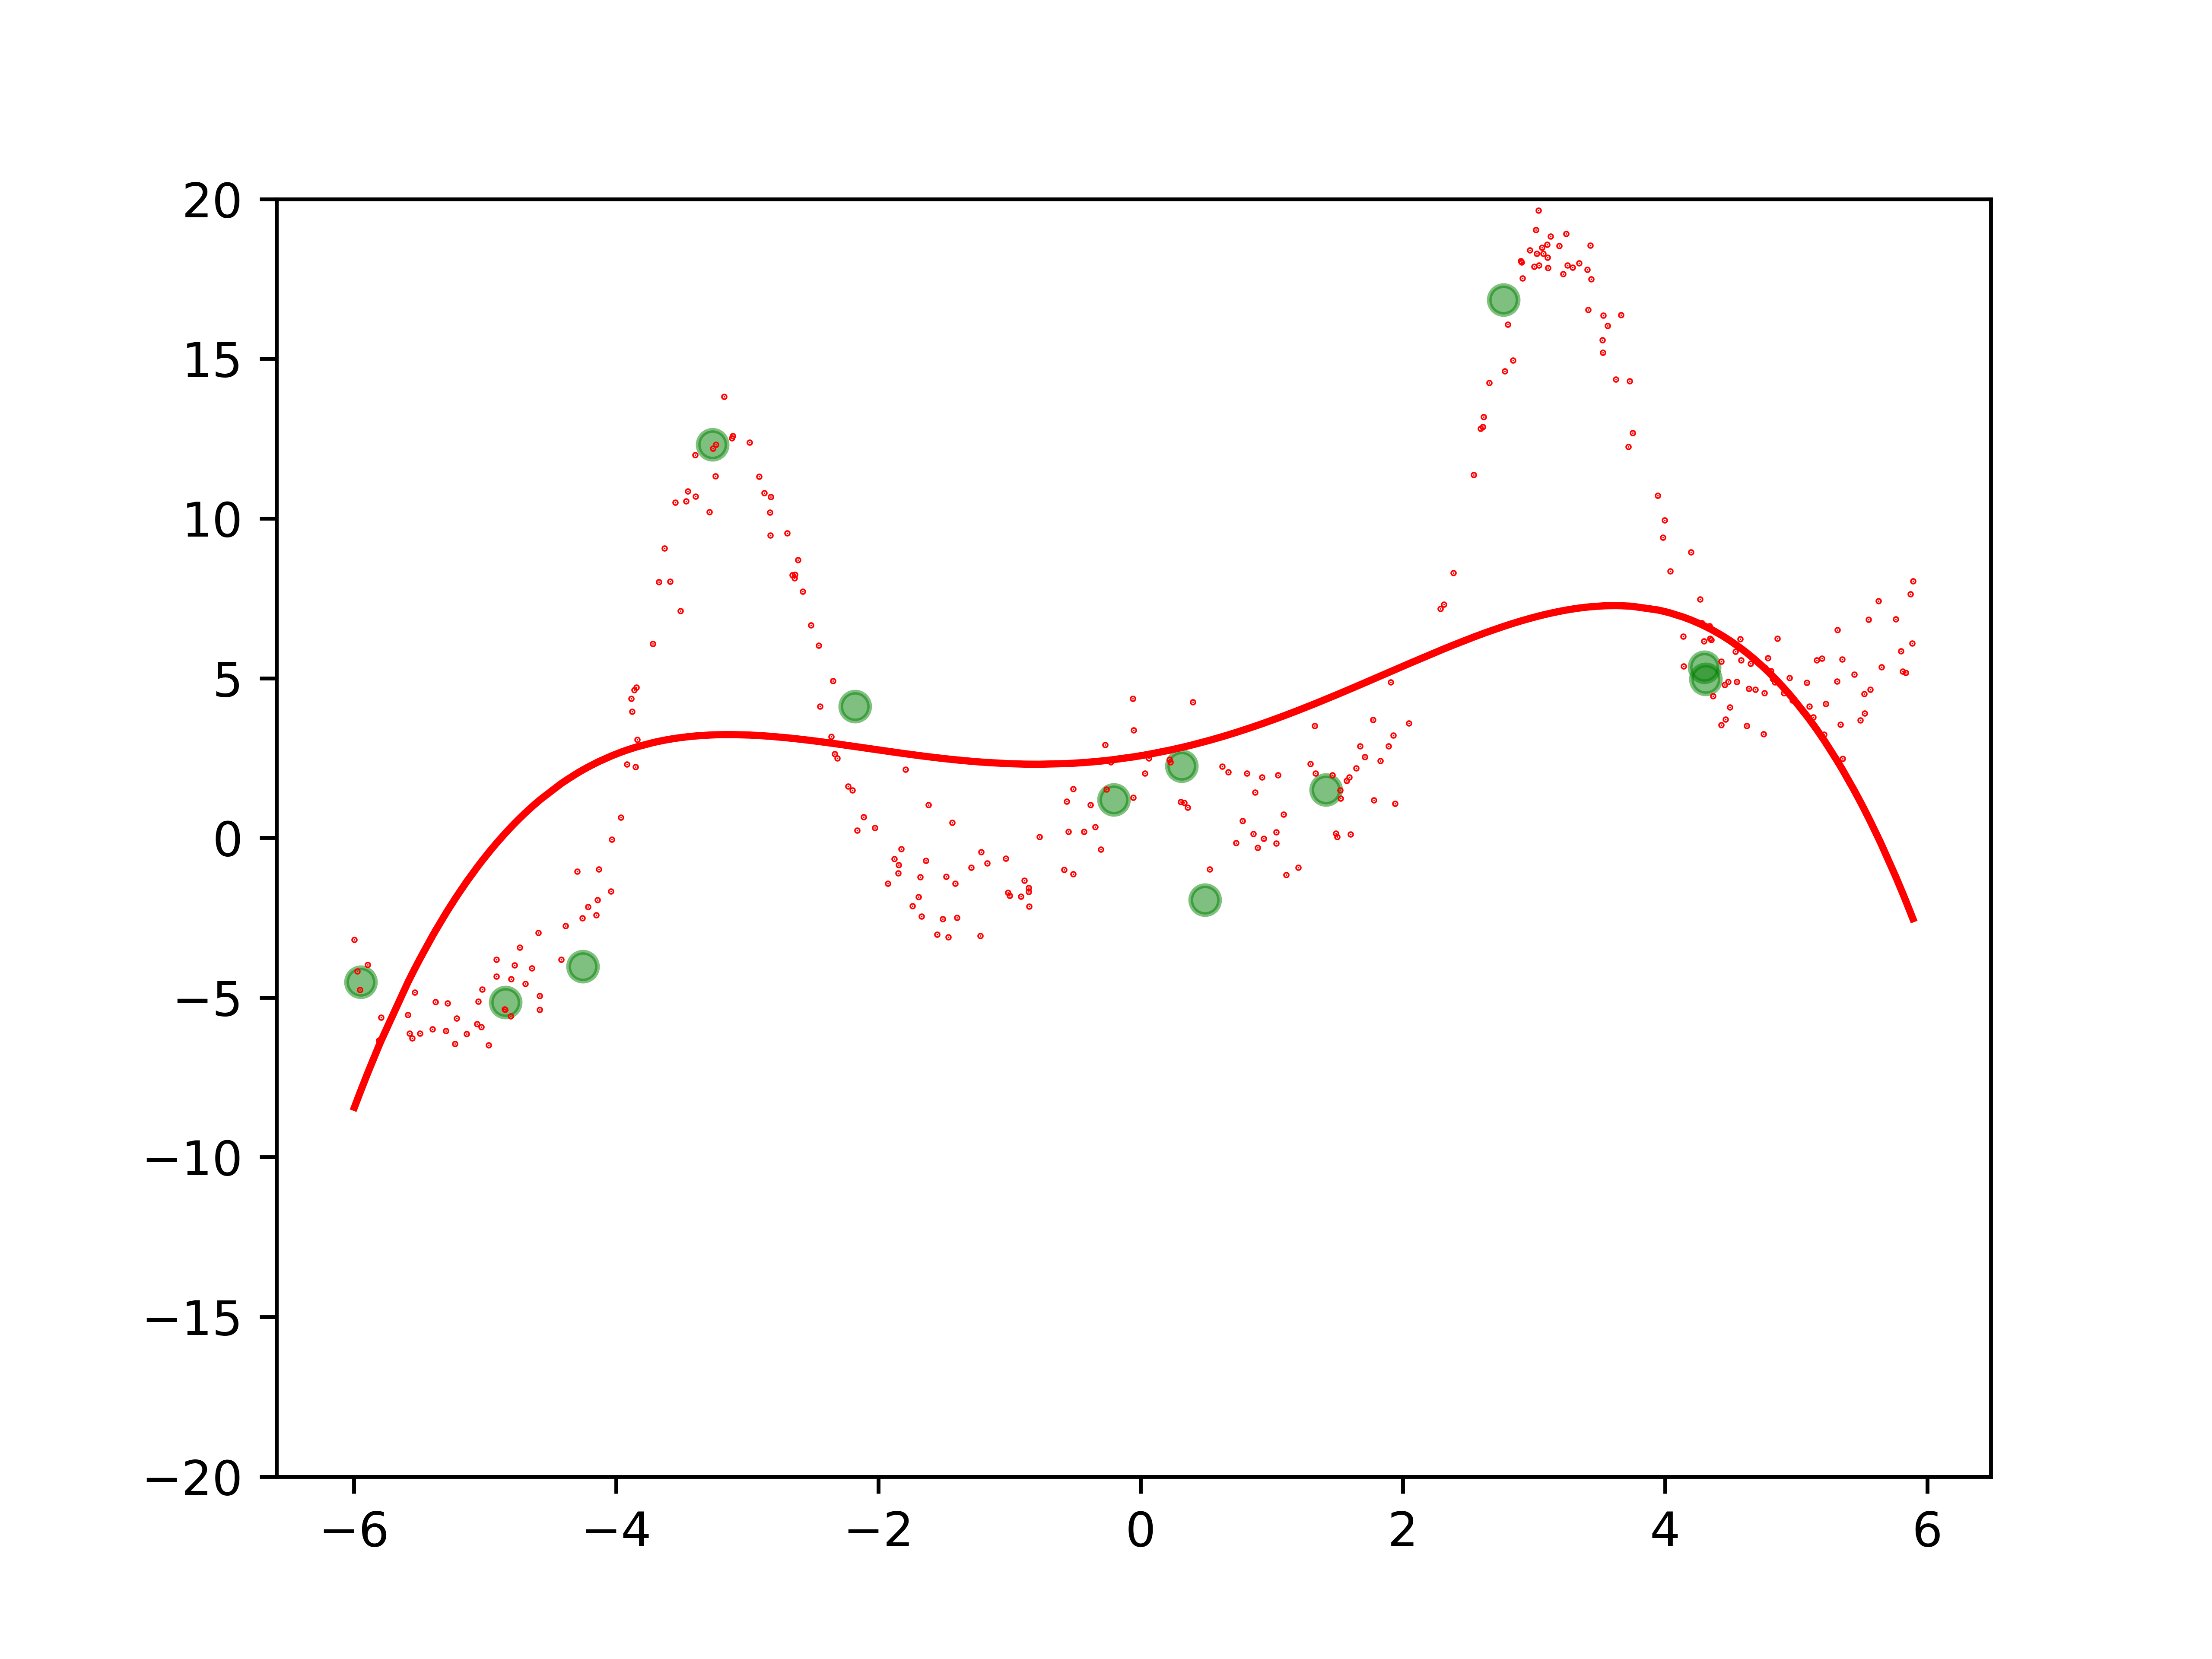
\includegraphics[scale=0.8]{fit_curve_polynomials.png}
        \caption{多项式拟合曲线}
    \end{figure}
    \paragraph{(3)}:
    以余弦多项式为基函数时,在训练集和测试集上的均方误差随$\lambda$的关系、拟合参数随$\lambda$的关系
    如表 3 所示。
    \begin{table}[htbp]
        \centering
        \label{poly-cos_params}
        \begin{tabular}[htbp]{cc}
            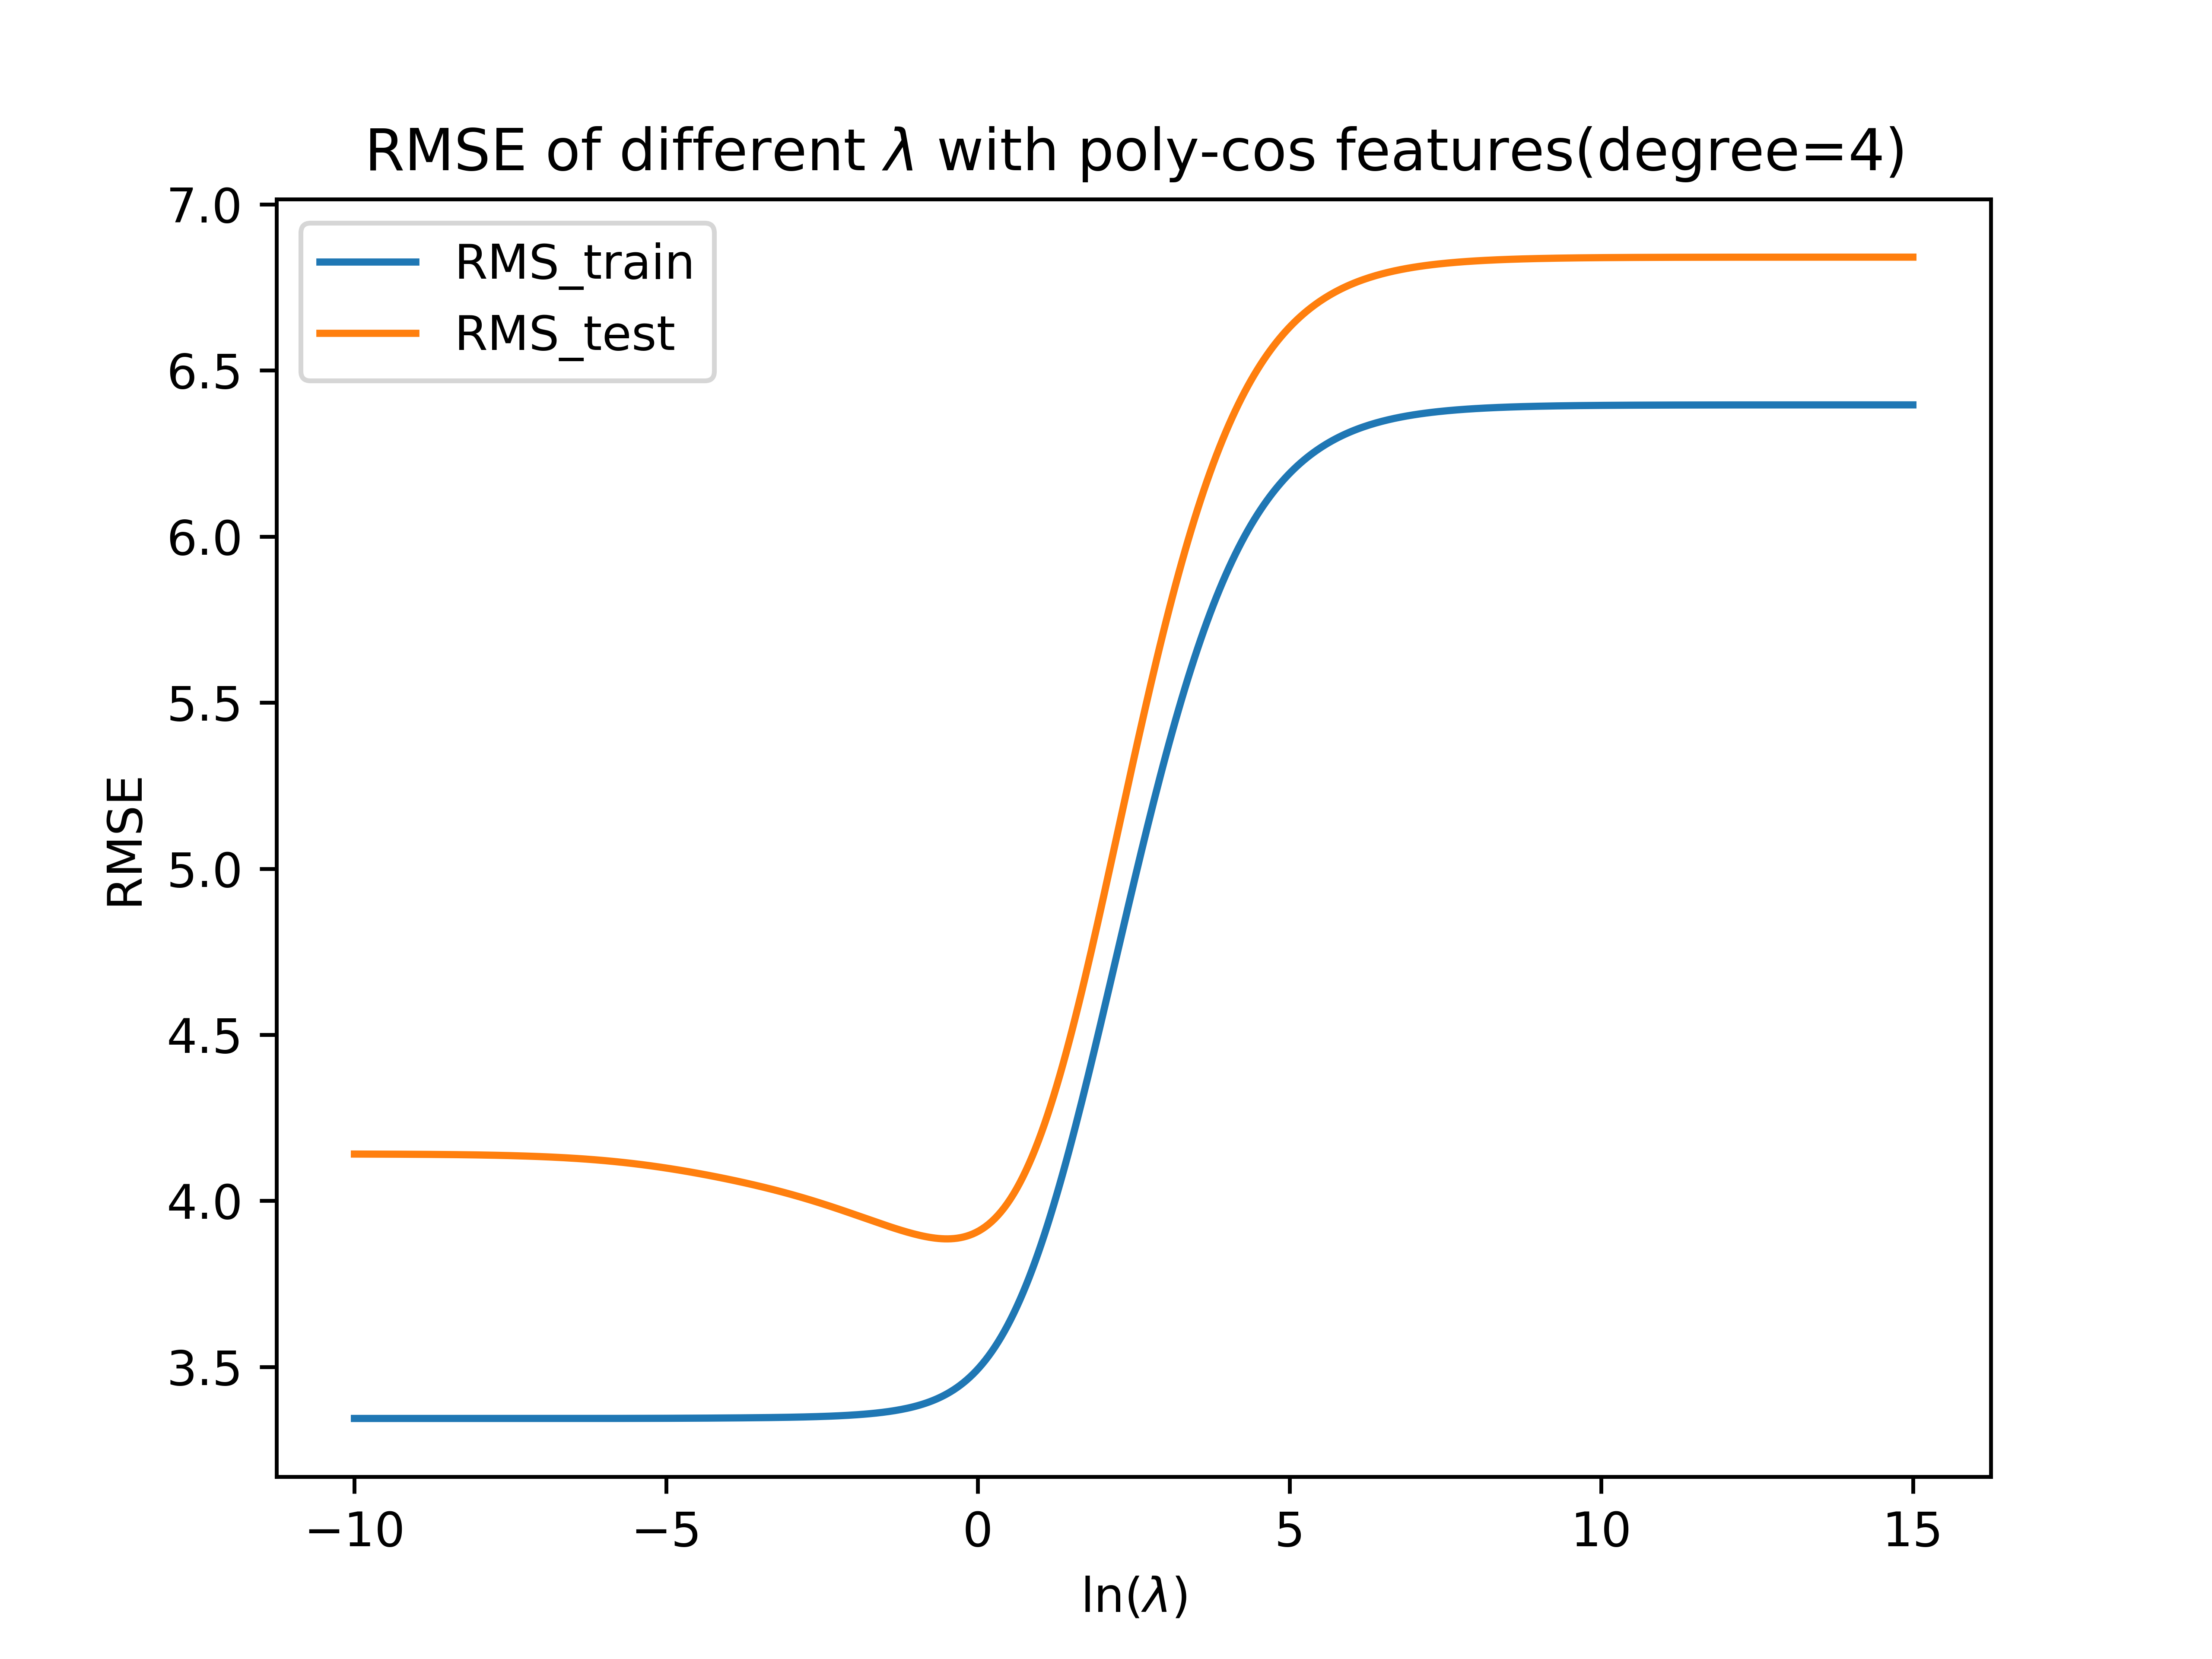
\includegraphics[scale=0.5]{RMSE_poly-cos.png} & 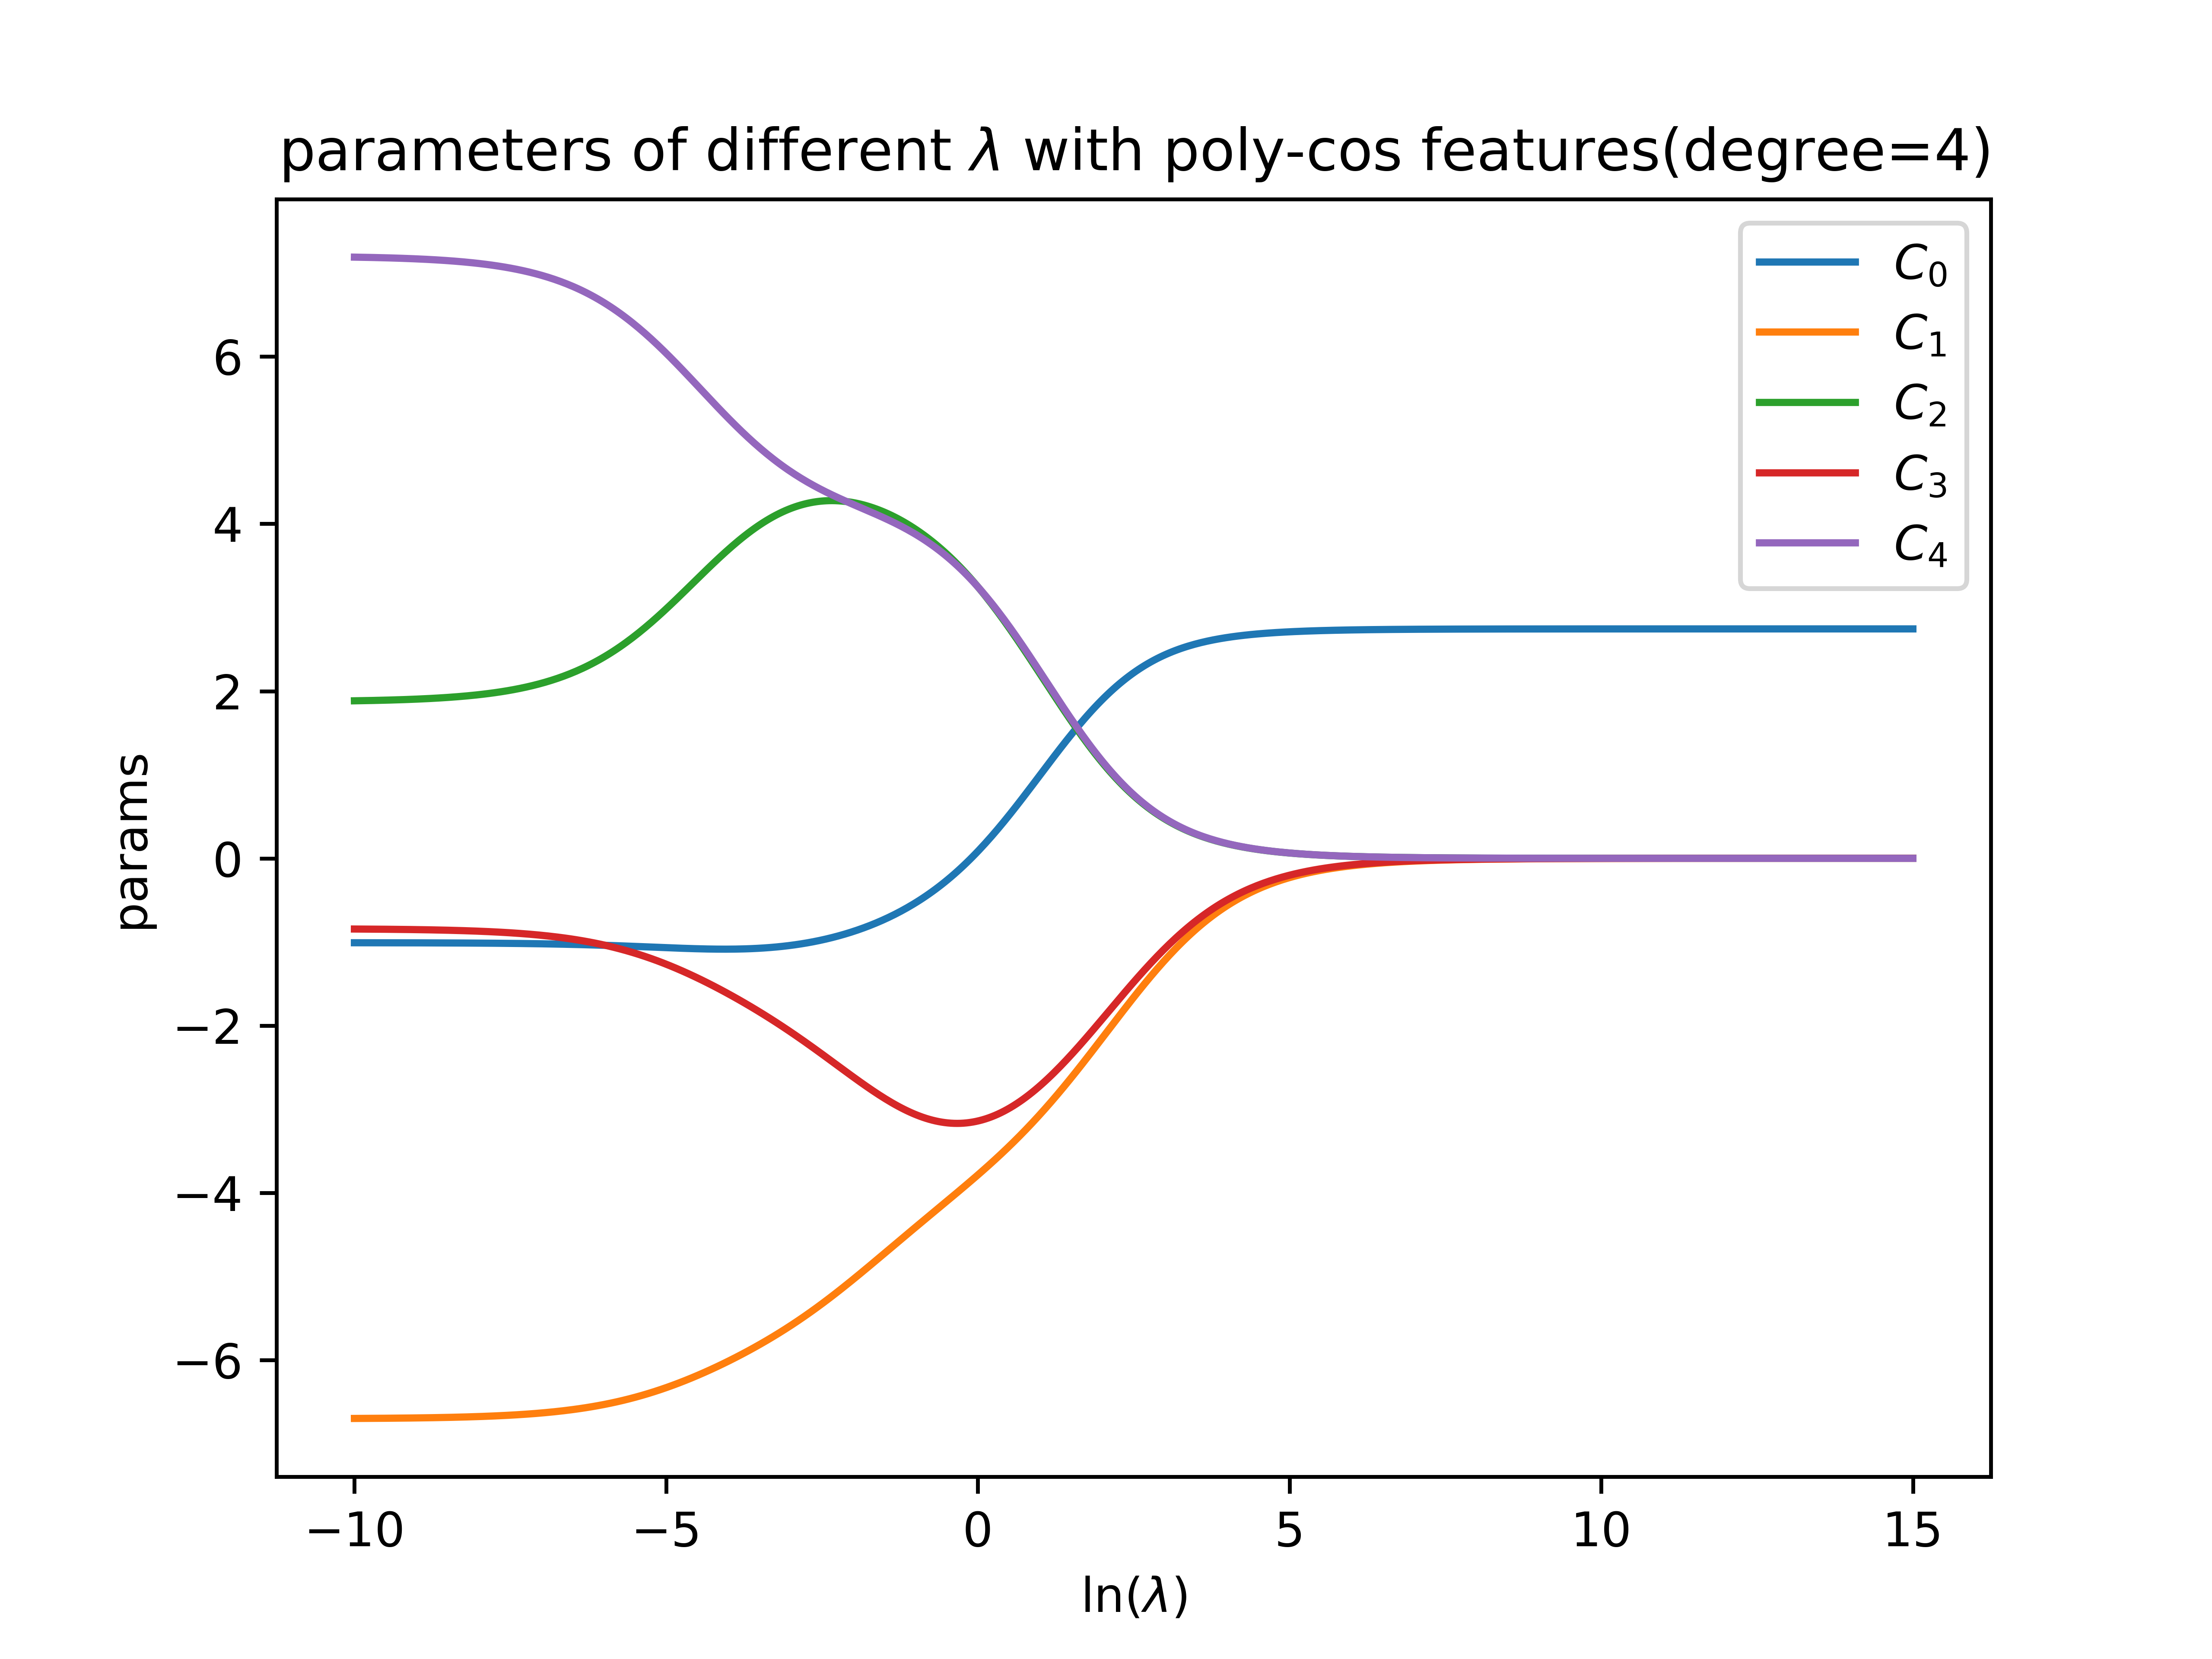
\includegraphics[scale=0.5]{Params_poly-cos.png} \\
        \end{tabular}
        \caption{余弦多项式为基函数时均方误差与拟合参数随超参数的关系}
    \end{table}
    \paragraph{(4)}:
    从表 3 可以看出,当$\ln(\lambda) = -0.5$左右时,可以在训练集和测试集上都得到一个比较小的
    均方误差,选定这个参数。得到表 4 的数据:
    \begin{table}[htbp]
        \centering
        \caption{最佳超参数下的余弦多项式拟合数据}
        \begin{tabular}[htbp]{ccccccc}
            \toprule
            RMSE-train & RMSE-test & $C_0$ & $C_1$ & $C_2$ & $C_3$ & $C_4$\\
            \midrule
            3.4184 & 3.8854 & -0.2650 & -4.1013 & 3.6405 & -3.1622 & 3.6111 \\
            \bottomrule
        \end{tabular}
        \label{poly-cos curve table}
    \end{table}
    同时给出拟合图像图 2。
    \begin{figure}[htbp]
        \centering
        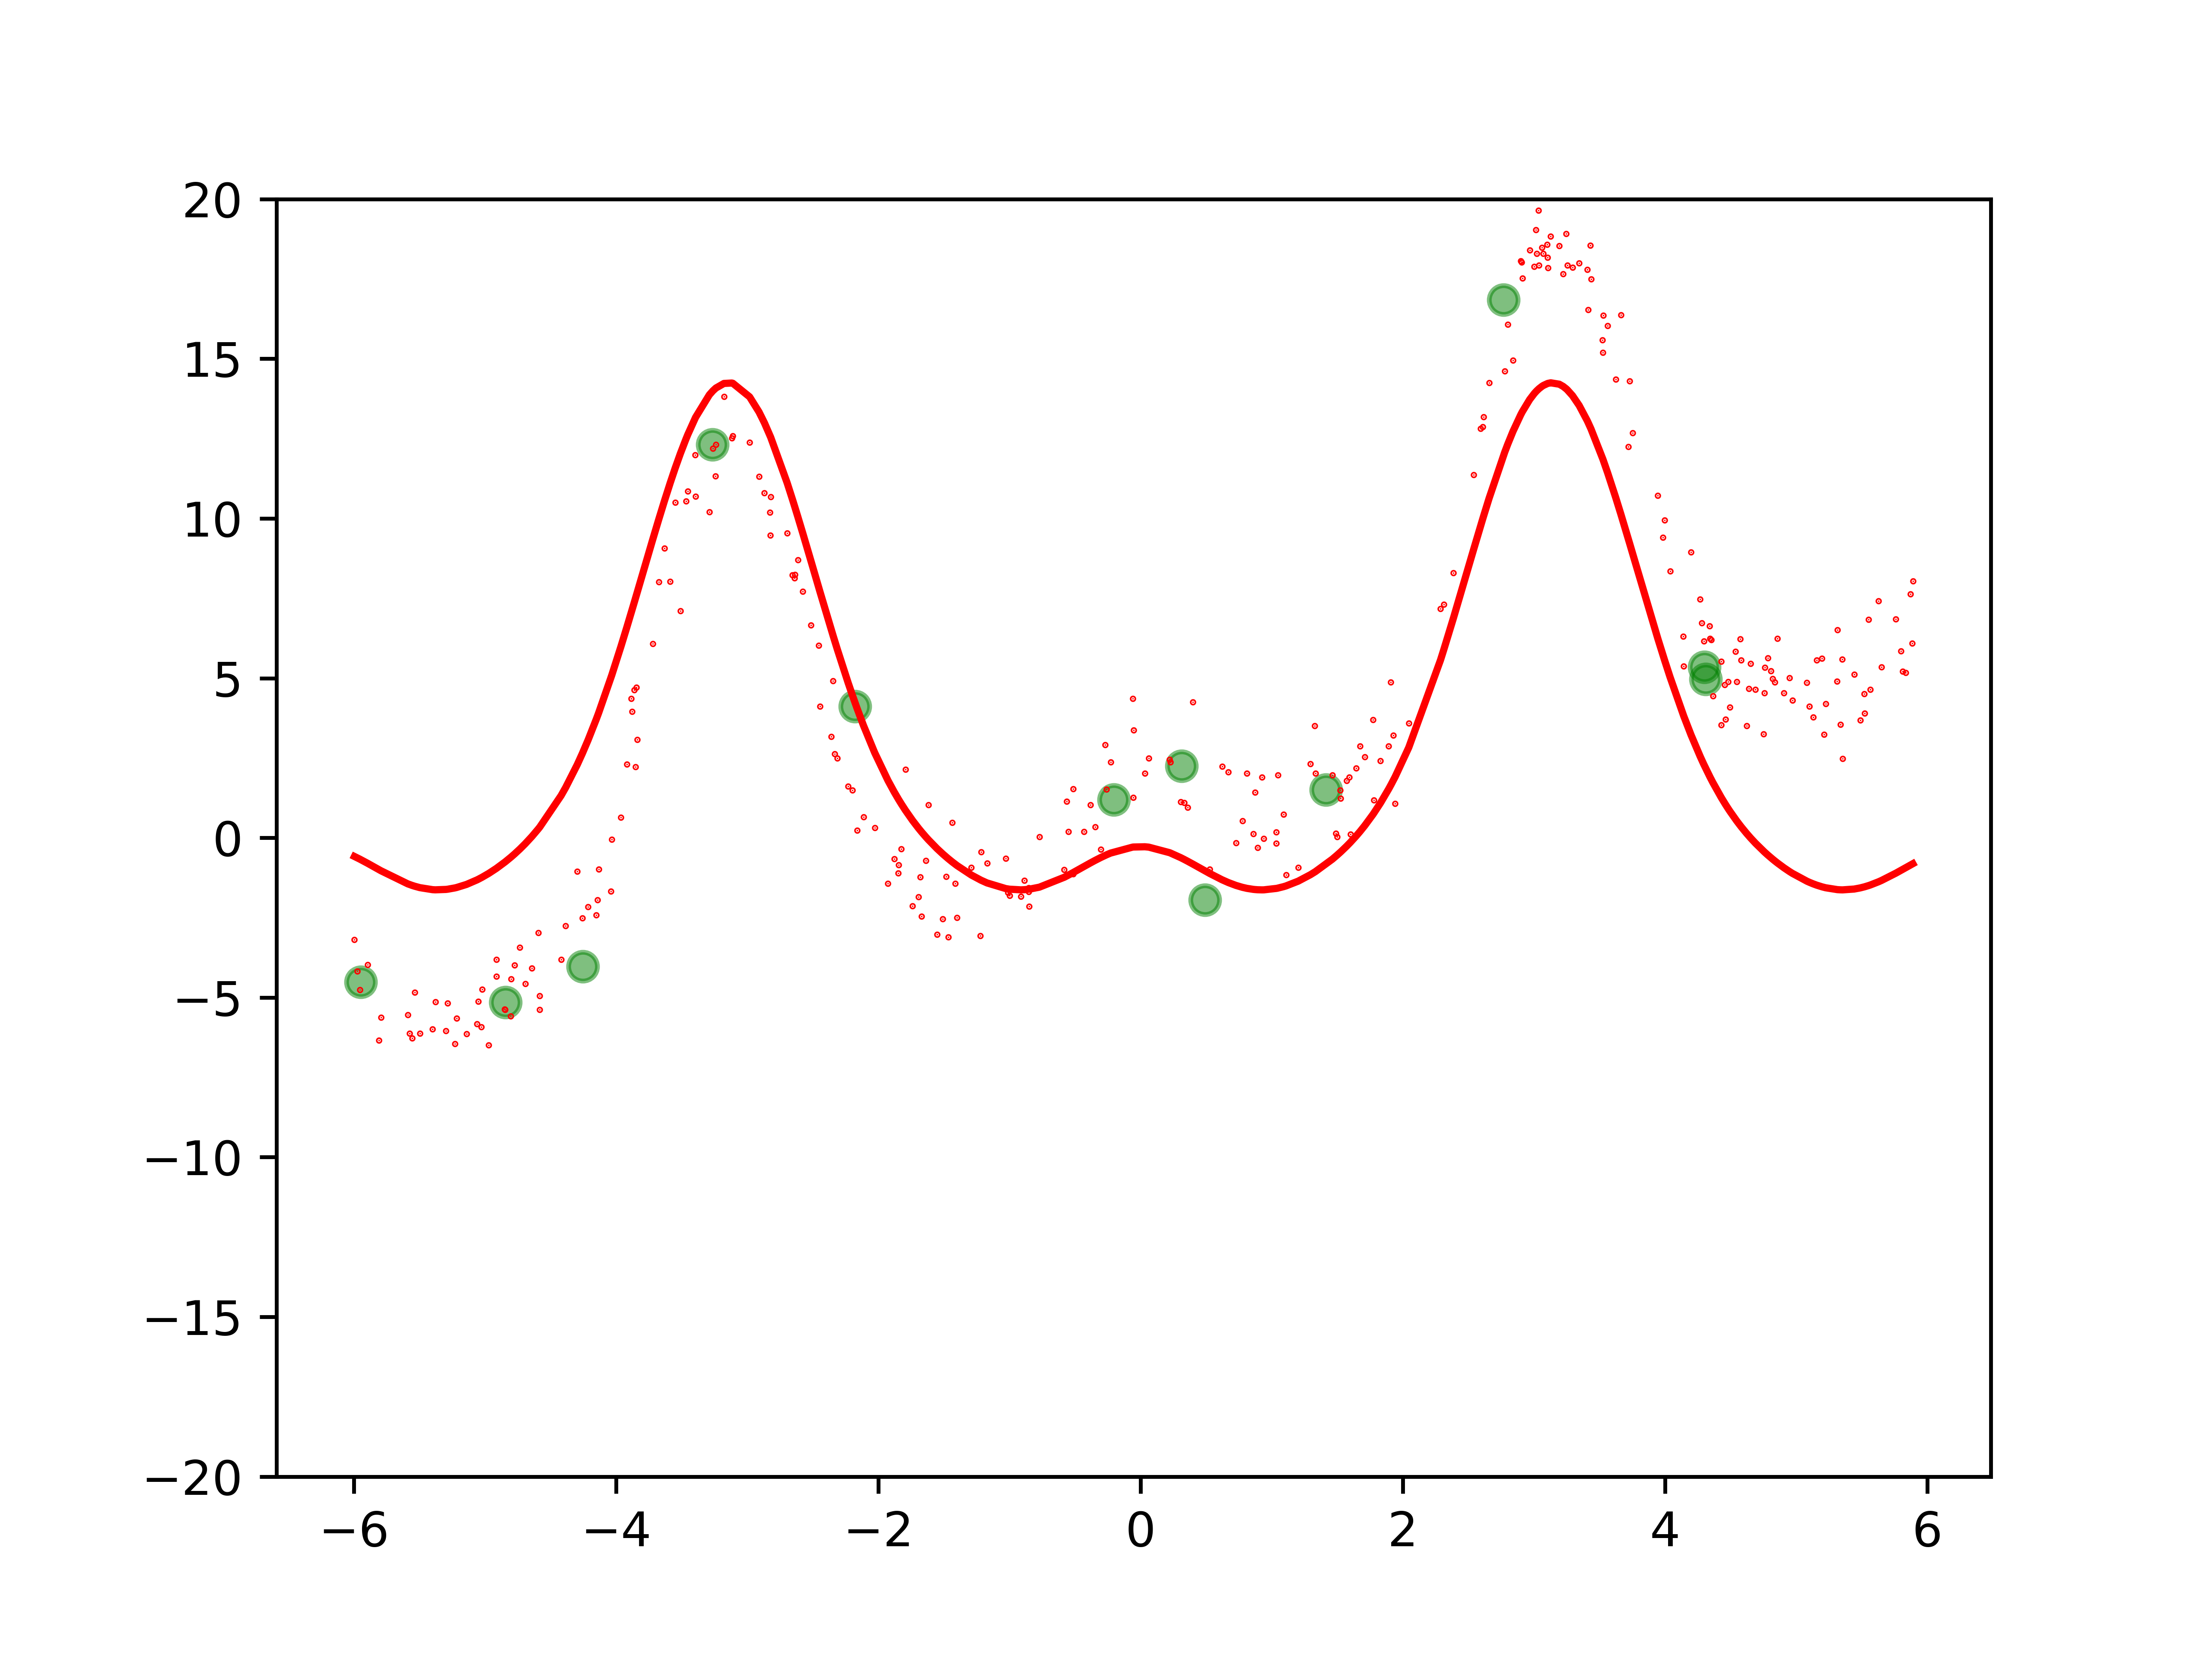
\includegraphics[scale=0.8]{fit_curve_poly-cos.png}
        \caption{余弦多项式拟合曲线}
    \end{figure}
    \paragraph{(5)}:
    将给定的拟合函数的$x$移项到等式左边,然后可以同样用余弦多项式拟合。
    在训练集和测试集上的均方误差随$\lambda$的关系、拟合参数随$\lambda$的关系
    如表 5 所示。
    \begin{table}[htbp]
        \centering
        \begin{tabular}[htbp]{cc}
            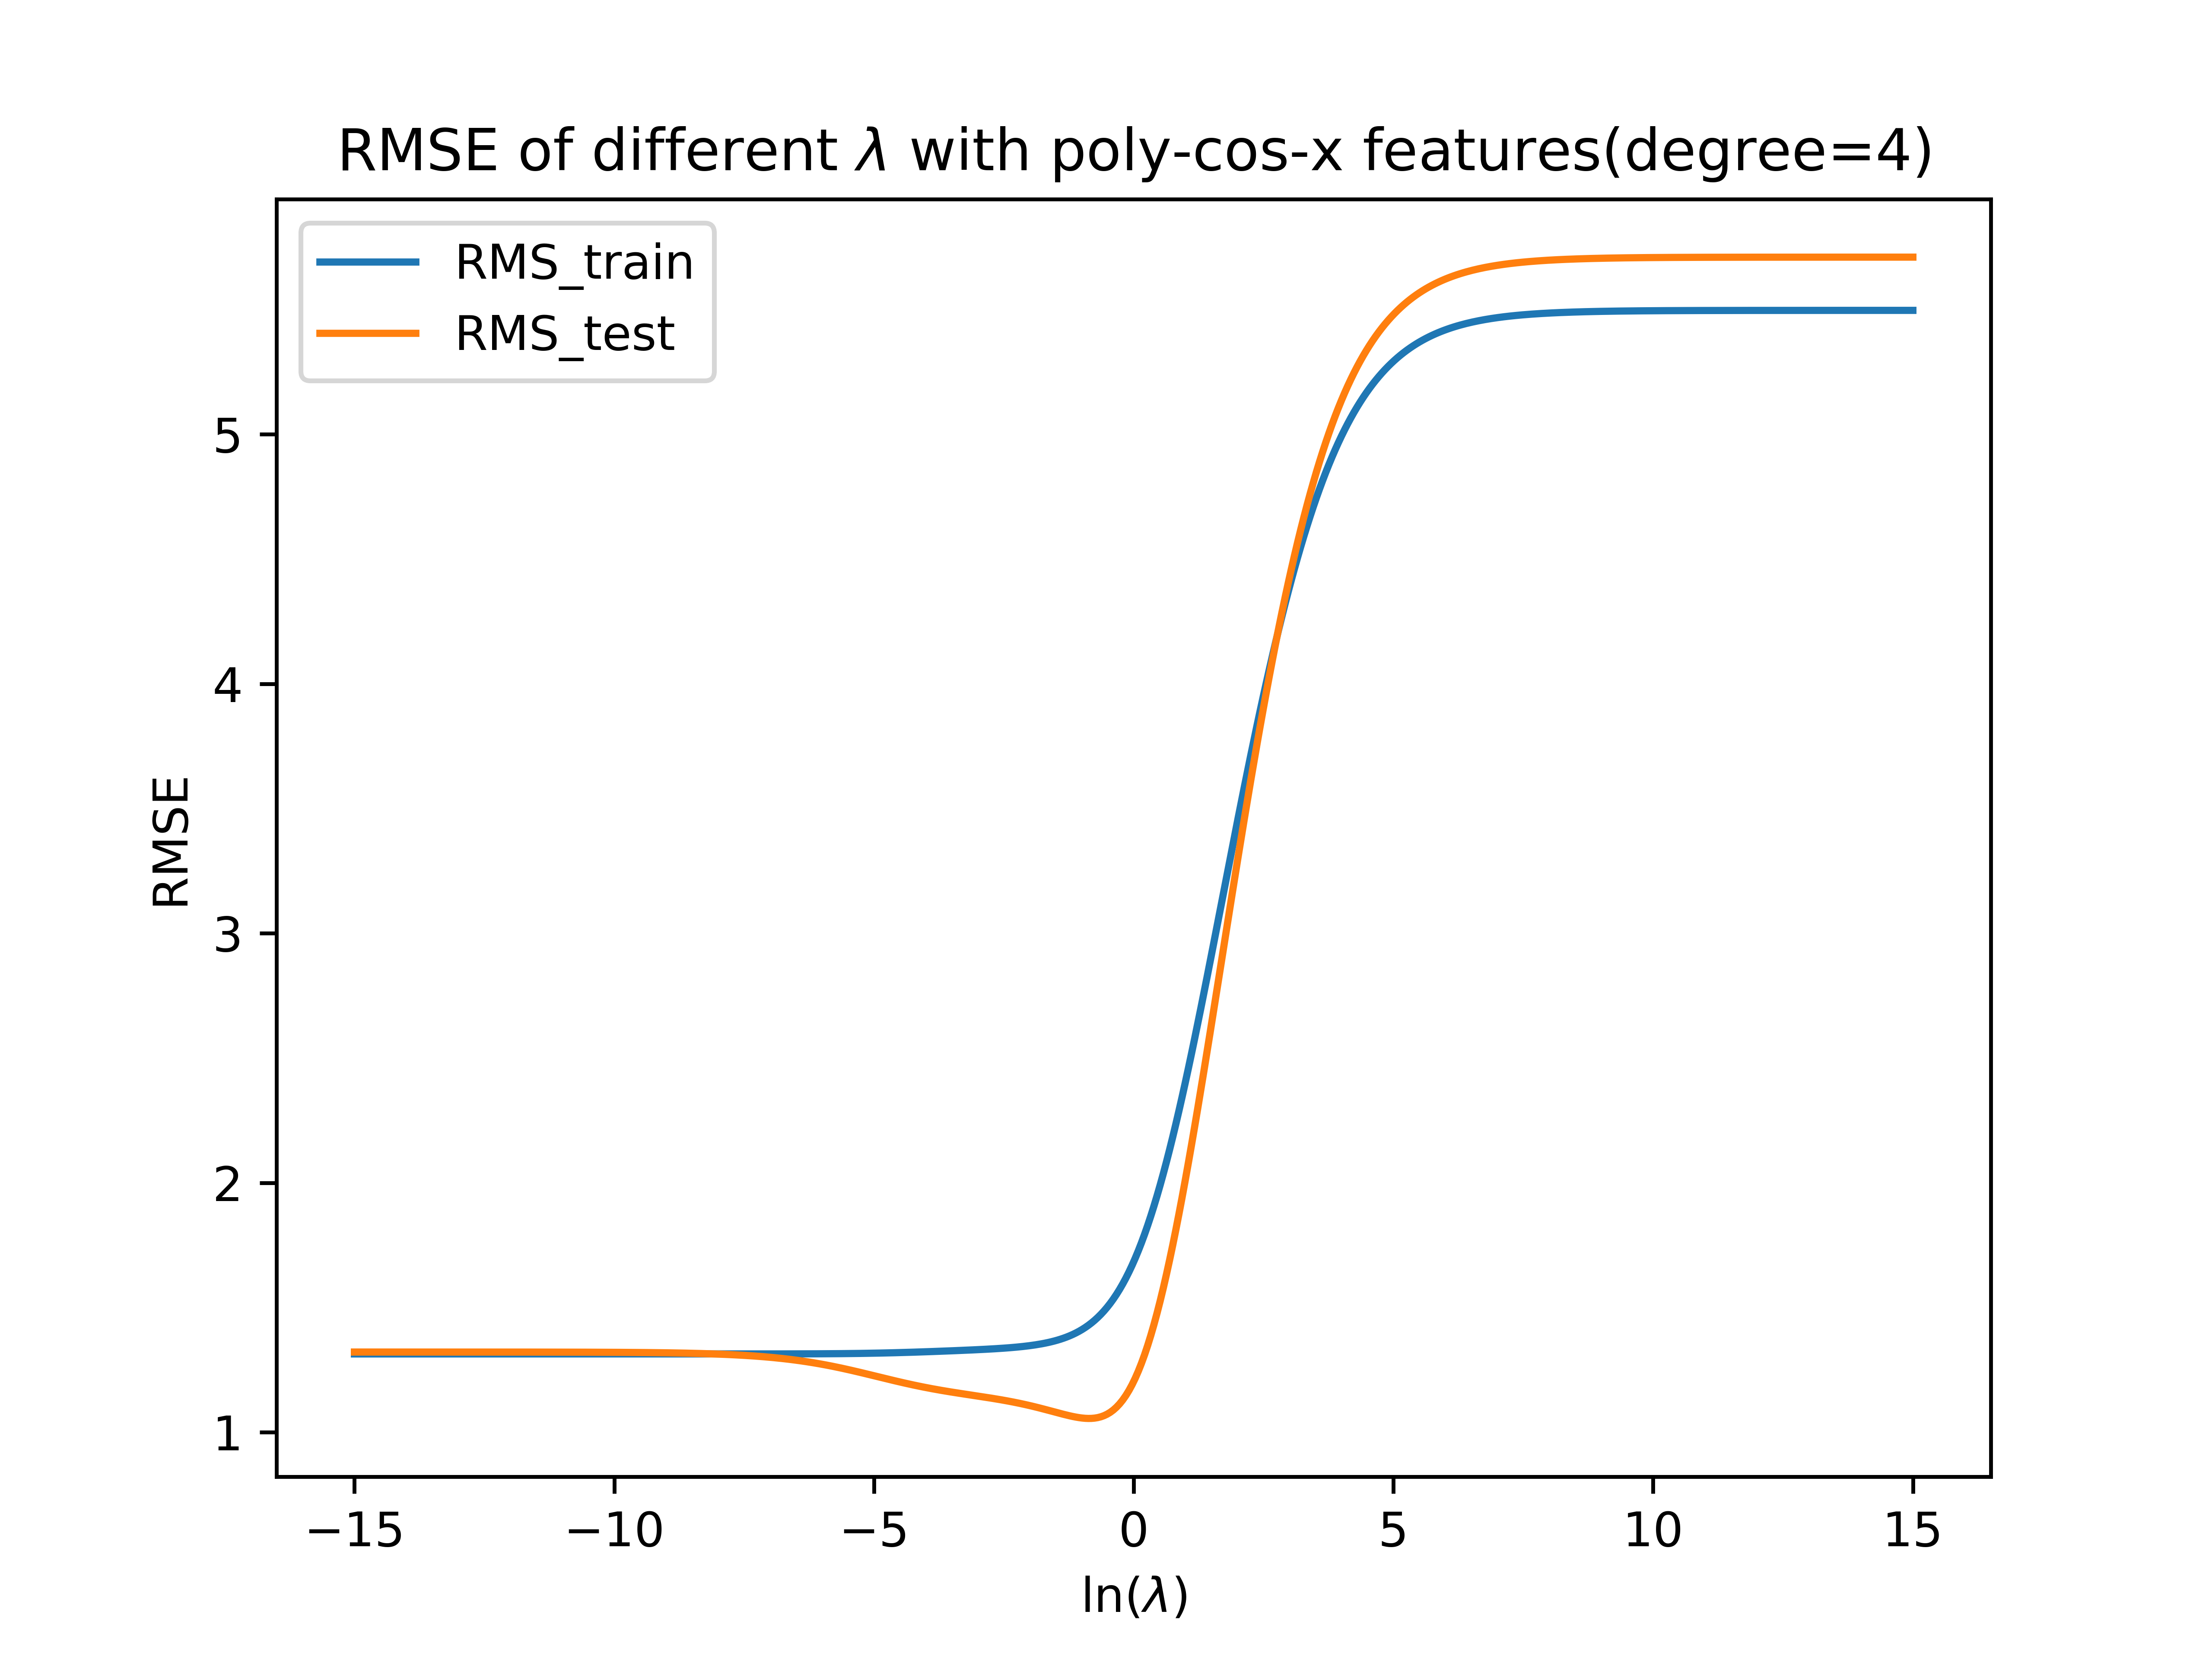
\includegraphics[scale=0.5]{RMSE_poly-cos-x.png} & 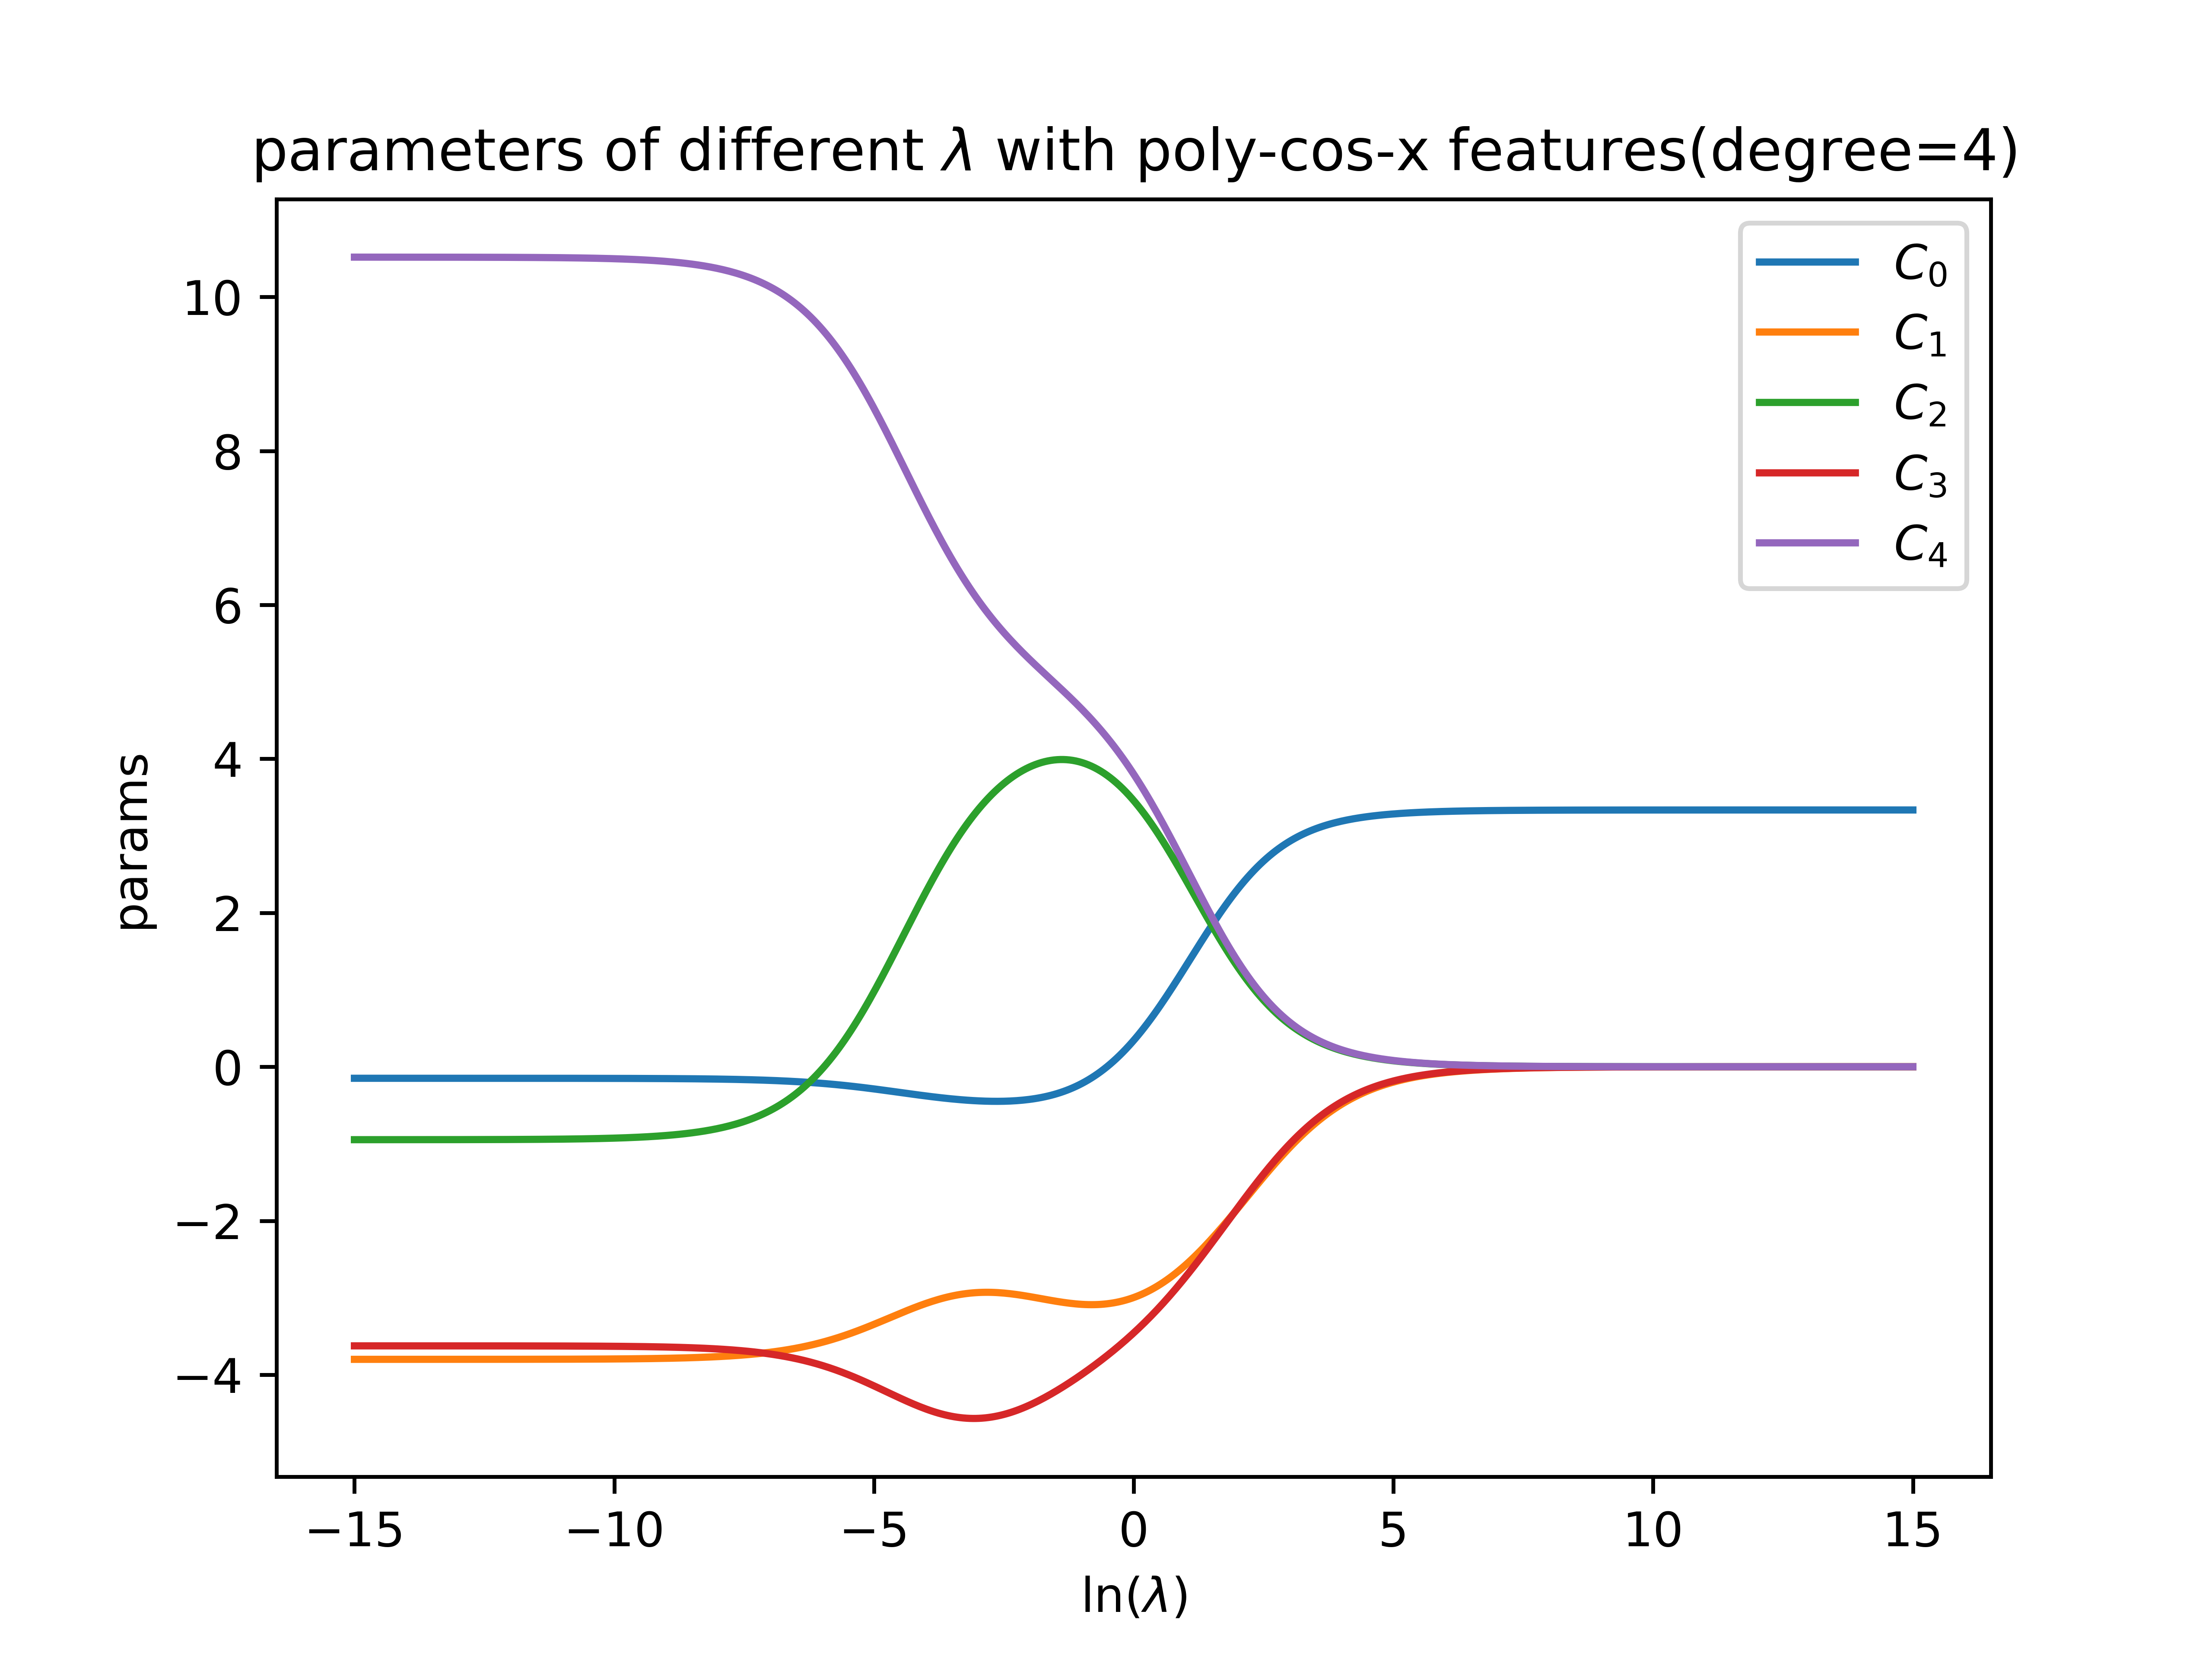
\includegraphics[scale=0.5]{Params_poly-cos-x.png} \\
        \end{tabular}
        \caption{余弦多项式+线性函数为基函数时均方误差与拟合参数随超参数的关系}
    \end{table}
    从表 5 可以看出,当$\ln(\lambda) = -0.5$左右时,可以在训练集和测试集上都得到一个比较小的
    均方误差,选定这个参数。得到表 6 的数据:
    \begin{table}[htbp]
        \centering
        \caption{最佳超参数下的余弦多项式拟合数据}
        \begin{tabular}[htbp]{ccccccc}
            \toprule
            RMSE-train & RMSE-test & $C_0$ & $C_1$ & $C_2$ & $C_3$ & $C_4$\\
            \midrule
            1.5036 & 1.0738 & 0.0075 & -3.0780 & 3.7790 & -3.7457 & 4.2670 \\
            \bottomrule
        \end{tabular}
    \end{table}
    同时给出拟合图像图 3。
    \begin{figure}[htbp]
        \centering
        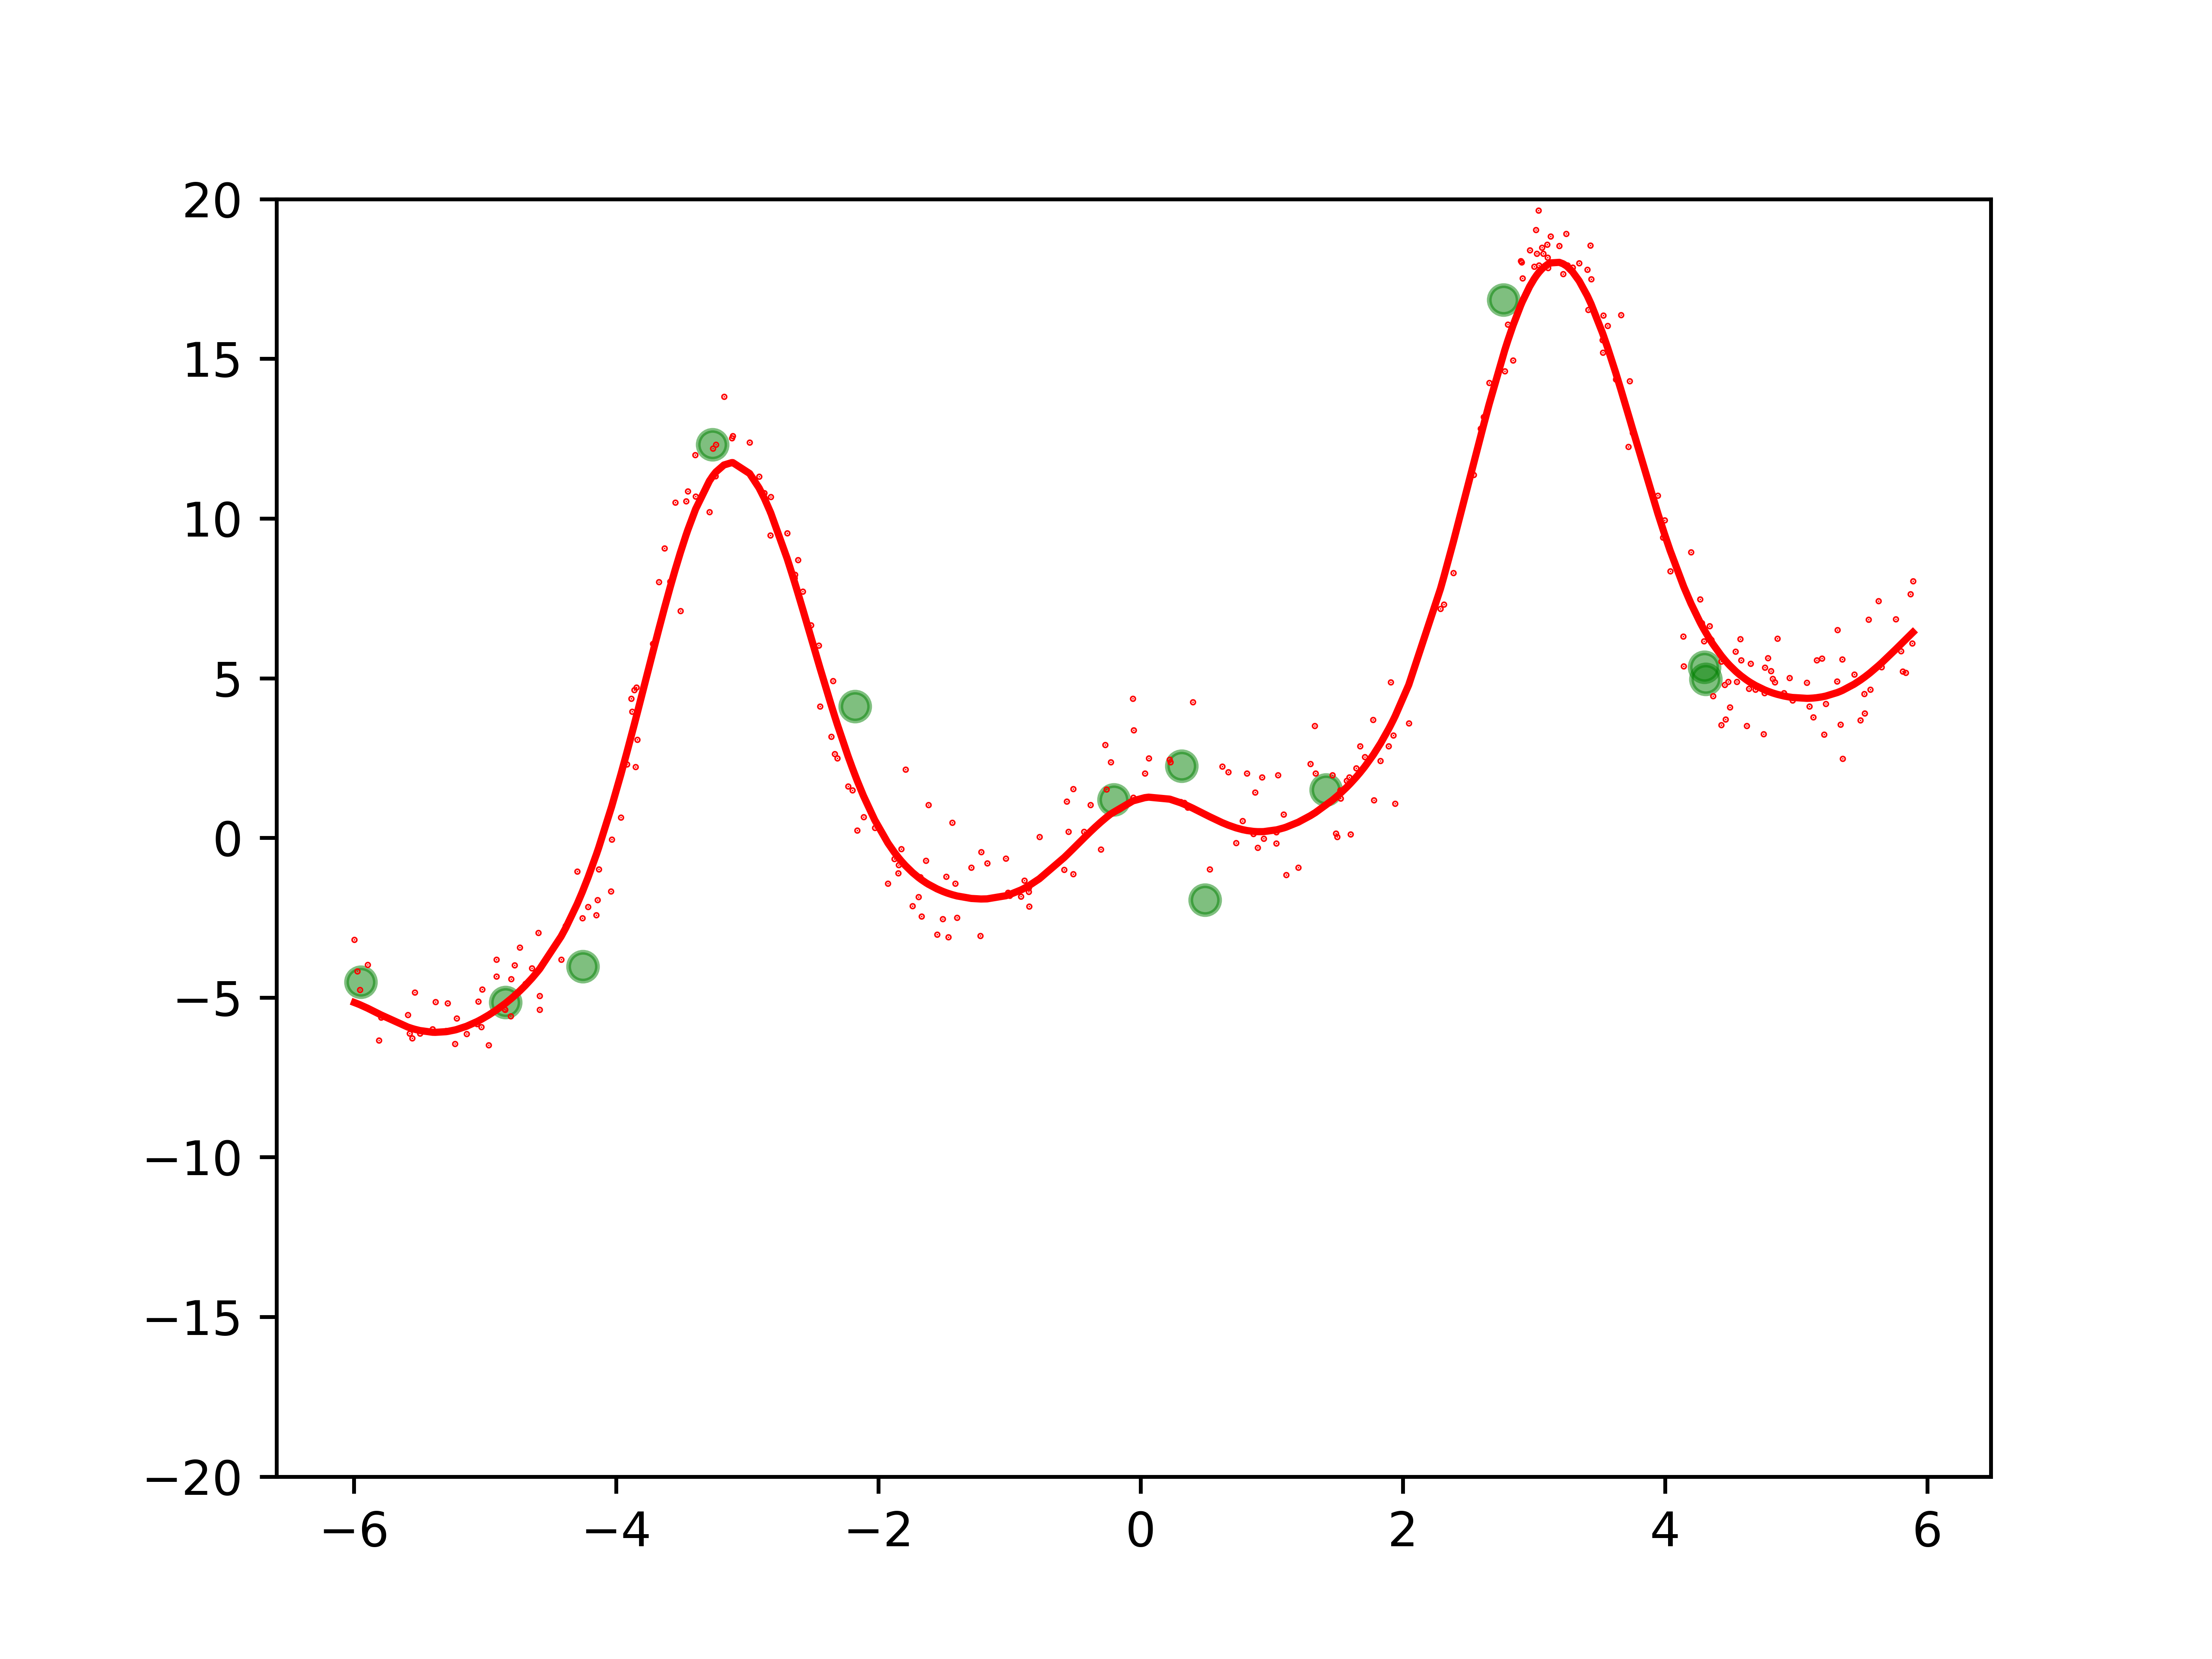
\includegraphics[scale=0.8]{fit_curve_poly-cos-x.png}
        \caption{余弦多项式+线性函数拟合曲线}
    \end{figure}
    \bibliographystyle{plain}
	\bibliography{ref}
\end{document}